% Options for packages loaded elsewhere
\PassOptionsToPackage{unicode}{hyperref}
\PassOptionsToPackage{hyphens}{url}
%
\documentclass[
  11pt,
]{article}
\usepackage{amsmath,amssymb}
\usepackage{lmodern}
\usepackage{iftex}
\ifPDFTeX
  \usepackage[T1]{fontenc}
  \usepackage[utf8]{inputenc}
  \usepackage{textcomp} % provide euro and other symbols
\else % if luatex or xetex
  \usepackage{unicode-math}
  \defaultfontfeatures{Scale=MatchLowercase}
  \defaultfontfeatures[\rmfamily]{Ligatures=TeX,Scale=1}
\fi
% Use upquote if available, for straight quotes in verbatim environments
\IfFileExists{upquote.sty}{\usepackage{upquote}}{}
\IfFileExists{microtype.sty}{% use microtype if available
  \usepackage[]{microtype}
  \UseMicrotypeSet[protrusion]{basicmath} % disable protrusion for tt fonts
}{}
\makeatletter
\@ifundefined{KOMAClassName}{% if non-KOMA class
  \IfFileExists{parskip.sty}{%
    \usepackage{parskip}
  }{% else
    \setlength{\parindent}{0pt}
    \setlength{\parskip}{6pt plus 2pt minus 1pt}}
}{% if KOMA class
  \KOMAoptions{parskip=half}}
\makeatother
\usepackage{xcolor}
\usepackage[margin=2cm]{geometry}
\usepackage{color}
\usepackage{fancyvrb}
\newcommand{\VerbBar}{|}
\newcommand{\VERB}{\Verb[commandchars=\\\{\}]}
\DefineVerbatimEnvironment{Highlighting}{Verbatim}{commandchars=\\\{\}}
% Add ',fontsize=\small' for more characters per line
\usepackage{framed}
\definecolor{shadecolor}{RGB}{248,248,248}
\newenvironment{Shaded}{\begin{snugshade}}{\end{snugshade}}
\newcommand{\AlertTok}[1]{\textcolor[rgb]{0.94,0.16,0.16}{#1}}
\newcommand{\AnnotationTok}[1]{\textcolor[rgb]{0.56,0.35,0.01}{\textbf{\textit{#1}}}}
\newcommand{\AttributeTok}[1]{\textcolor[rgb]{0.77,0.63,0.00}{#1}}
\newcommand{\BaseNTok}[1]{\textcolor[rgb]{0.00,0.00,0.81}{#1}}
\newcommand{\BuiltInTok}[1]{#1}
\newcommand{\CharTok}[1]{\textcolor[rgb]{0.31,0.60,0.02}{#1}}
\newcommand{\CommentTok}[1]{\textcolor[rgb]{0.56,0.35,0.01}{\textit{#1}}}
\newcommand{\CommentVarTok}[1]{\textcolor[rgb]{0.56,0.35,0.01}{\textbf{\textit{#1}}}}
\newcommand{\ConstantTok}[1]{\textcolor[rgb]{0.00,0.00,0.00}{#1}}
\newcommand{\ControlFlowTok}[1]{\textcolor[rgb]{0.13,0.29,0.53}{\textbf{#1}}}
\newcommand{\DataTypeTok}[1]{\textcolor[rgb]{0.13,0.29,0.53}{#1}}
\newcommand{\DecValTok}[1]{\textcolor[rgb]{0.00,0.00,0.81}{#1}}
\newcommand{\DocumentationTok}[1]{\textcolor[rgb]{0.56,0.35,0.01}{\textbf{\textit{#1}}}}
\newcommand{\ErrorTok}[1]{\textcolor[rgb]{0.64,0.00,0.00}{\textbf{#1}}}
\newcommand{\ExtensionTok}[1]{#1}
\newcommand{\FloatTok}[1]{\textcolor[rgb]{0.00,0.00,0.81}{#1}}
\newcommand{\FunctionTok}[1]{\textcolor[rgb]{0.00,0.00,0.00}{#1}}
\newcommand{\ImportTok}[1]{#1}
\newcommand{\InformationTok}[1]{\textcolor[rgb]{0.56,0.35,0.01}{\textbf{\textit{#1}}}}
\newcommand{\KeywordTok}[1]{\textcolor[rgb]{0.13,0.29,0.53}{\textbf{#1}}}
\newcommand{\NormalTok}[1]{#1}
\newcommand{\OperatorTok}[1]{\textcolor[rgb]{0.81,0.36,0.00}{\textbf{#1}}}
\newcommand{\OtherTok}[1]{\textcolor[rgb]{0.56,0.35,0.01}{#1}}
\newcommand{\PreprocessorTok}[1]{\textcolor[rgb]{0.56,0.35,0.01}{\textit{#1}}}
\newcommand{\RegionMarkerTok}[1]{#1}
\newcommand{\SpecialCharTok}[1]{\textcolor[rgb]{0.00,0.00,0.00}{#1}}
\newcommand{\SpecialStringTok}[1]{\textcolor[rgb]{0.31,0.60,0.02}{#1}}
\newcommand{\StringTok}[1]{\textcolor[rgb]{0.31,0.60,0.02}{#1}}
\newcommand{\VariableTok}[1]{\textcolor[rgb]{0.00,0.00,0.00}{#1}}
\newcommand{\VerbatimStringTok}[1]{\textcolor[rgb]{0.31,0.60,0.02}{#1}}
\newcommand{\WarningTok}[1]{\textcolor[rgb]{0.56,0.35,0.01}{\textbf{\textit{#1}}}}
\usepackage{longtable,booktabs,array}
\usepackage{calc} % for calculating minipage widths
% Correct order of tables after \paragraph or \subparagraph
\usepackage{etoolbox}
\makeatletter
\patchcmd\longtable{\par}{\if@noskipsec\mbox{}\fi\par}{}{}
\makeatother
% Allow footnotes in longtable head/foot
\IfFileExists{footnotehyper.sty}{\usepackage{footnotehyper}}{\usepackage{footnote}}
\makesavenoteenv{longtable}
\usepackage{graphicx}
\makeatletter
\def\maxwidth{\ifdim\Gin@nat@width>\linewidth\linewidth\else\Gin@nat@width\fi}
\def\maxheight{\ifdim\Gin@nat@height>\textheight\textheight\else\Gin@nat@height\fi}
\makeatother
% Scale images if necessary, so that they will not overflow the page
% margins by default, and it is still possible to overwrite the defaults
% using explicit options in \includegraphics[width, height, ...]{}
\setkeys{Gin}{width=\maxwidth,height=\maxheight,keepaspectratio}
% Set default figure placement to htbp
\makeatletter
\def\fps@figure{htbp}
\makeatother
\setlength{\emergencystretch}{3em} % prevent overfull lines
\providecommand{\tightlist}{%
  \setlength{\itemsep}{0pt}\setlength{\parskip}{0pt}}
\setcounter{secnumdepth}{-\maxdimen} % remove section numbering
\ifLuaTeX
  \usepackage{selnolig}  % disable illegal ligatures
\fi
\IfFileExists{bookmark.sty}{\usepackage{bookmark}}{\usepackage{hyperref}}
\IfFileExists{xurl.sty}{\usepackage{xurl}}{} % add URL line breaks if available
\urlstyle{same} % disable monospaced font for URLs
\hypersetup{
  pdftitle={ABE6933 SML Take-Home Final Exam (100 pts + 10 pts bonus)},
  pdfauthor={Christopher Marais},
  hidelinks,
  pdfcreator={LaTeX via pandoc}}

\title{ABE6933 SML Take-Home Final Exam (100 pts + 10 pts bonus)}
\author{Christopher Marais}
\date{}

\begin{document}
\maketitle

\hypertarget{exam-code-data-and-libraries}{%
\section{Exam code, data, and
libraries}\label{exam-code-data-and-libraries}}

\begin{Shaded}
\begin{Highlighting}[]
\CommentTok{\# functions}
\NormalTok{myCVids }\OtherTok{\textless{}{-}} \ControlFlowTok{function}\NormalTok{(n, K, }\AttributeTok{seed=}\DecValTok{0}\NormalTok{) \{}
\CommentTok{\# balanced subsets generation (subset sizes differ by at most 1)}
\CommentTok{\# n is the number of observations/rows in the training set}
\CommentTok{\# K is the desired number of folds (e.g., 5 or 10)}
\FunctionTok{set.seed}\NormalTok{(seed);}
\NormalTok{t }\OtherTok{=} \FunctionTok{floor}\NormalTok{(n}\SpecialCharTok{/}\NormalTok{K); r }\OtherTok{=}\NormalTok{ n}\SpecialCharTok{{-}}\NormalTok{t}\SpecialCharTok{*}\NormalTok{K;}
\NormalTok{id0 }\OtherTok{=} \FunctionTok{rep}\NormalTok{((}\DecValTok{1}\SpecialCharTok{:}\NormalTok{K),}\AttributeTok{times=}\NormalTok{t)}
\NormalTok{ids }\OtherTok{=} \FunctionTok{sample}\NormalTok{(id0,t}\SpecialCharTok{*}\NormalTok{K)}
\ControlFlowTok{if}\NormalTok{ (r }\SpecialCharTok{\textgreater{}} \DecValTok{0}\NormalTok{) \{ids }\OtherTok{=} \FunctionTok{c}\NormalTok{(ids, }\FunctionTok{sample}\NormalTok{(K,r))\}}
\NormalTok{ids}
\NormalTok{\}}

\CommentTok{\# function to generate all subsets of the set (1,2,...,p)}
\NormalTok{myf }\OtherTok{\textless{}{-}} \ControlFlowTok{function}\NormalTok{(p) \{}
\NormalTok{  out }\OtherTok{=} \FunctionTok{matrix}\NormalTok{(}\FunctionTok{c}\NormalTok{(}\DecValTok{0}\NormalTok{,}\DecValTok{1}\NormalTok{),}\AttributeTok{nrow=}\DecValTok{2}\NormalTok{);}
  \ControlFlowTok{if}\NormalTok{ (p }\SpecialCharTok{\textgreater{}} \DecValTok{1}\NormalTok{) \{}
    \ControlFlowTok{for}\NormalTok{ (i }\ControlFlowTok{in}\NormalTok{ (}\DecValTok{1}\SpecialCharTok{:}\NormalTok{(p}\DecValTok{{-}1}\NormalTok{))) \{}
\NormalTok{      d }\OtherTok{=} \DecValTok{2}\SpecialCharTok{\^{}}\NormalTok{i}
\NormalTok{      o1 }\OtherTok{=} \FunctionTok{cbind}\NormalTok{(}\FunctionTok{rep}\NormalTok{(}\DecValTok{0}\NormalTok{,d),out)}
\NormalTok{      o2 }\OtherTok{=} \FunctionTok{cbind}\NormalTok{(}\FunctionTok{rep}\NormalTok{(}\DecValTok{1}\NormalTok{,d),out)}
\NormalTok{      out }\OtherTok{=} \FunctionTok{rbind}\NormalTok{(o1,o2)}
\NormalTok{    \}}
\NormalTok{  \}}
  \FunctionTok{colnames}\NormalTok{(out) }\OtherTok{\textless{}{-}} \FunctionTok{c}\NormalTok{(}\DecValTok{2}\SpecialCharTok{\^{}}\NormalTok{((p}\DecValTok{{-}1}\NormalTok{)}\SpecialCharTok{:}\DecValTok{0}\NormalTok{)); }\CommentTok{\# powers for binary expansion}
  \CommentTok{\# colnames(out) \textless{}{-} c()}
\NormalTok{  out}
\NormalTok{\}}

\NormalTok{nbSubsets }\OtherTok{\textless{}{-}} \ControlFlowTok{function}\NormalTok{(p,m) \{}
\NormalTok{  M  }\OtherTok{=} \FunctionTok{myf}\NormalTok{(p)}
\NormalTok{  rs }\OtherTok{=} \FunctionTok{rowSums}\NormalTok{(M)}
\NormalTok{  ii }\OtherTok{=}\NormalTok{ (rs }\SpecialCharTok{==}\NormalTok{ m)}
\NormalTok{  (M[ii,])}
\NormalTok{\}}

\CommentTok{\# function to convert binary representation to decimal representation }
\NormalTok{bin2dec }\OtherTok{\textless{}{-}} \ControlFlowTok{function}\NormalTok{(binM) \{}
\NormalTok{  dd }\OtherTok{=} \FunctionTok{dim}\NormalTok{(binM);  }\CommentTok{\# nrows and ncols}
\NormalTok{  p }\OtherTok{=}\NormalTok{ dd[}\DecValTok{2}\NormalTok{]}\SpecialCharTok{{-}}\DecValTok{1}      \CommentTok{\# max power; }
\NormalTok{  d }\OtherTok{=} \FunctionTok{rep}\NormalTok{(}\DecValTok{0}\NormalTok{,dd[}\DecValTok{1}\NormalTok{]) }\CommentTok{\# initialize placeholder for the answer}
  \ControlFlowTok{for}\NormalTok{ (i }\ControlFlowTok{in} \DecValTok{1}\SpecialCharTok{:}\NormalTok{(p}\SpecialCharTok{+}\DecValTok{1}\NormalTok{)) \{}
\NormalTok{    d }\OtherTok{=}\NormalTok{ d }\SpecialCharTok{+} \DecValTok{2}\SpecialCharTok{\^{}}\NormalTok{(p}\SpecialCharTok{+}\DecValTok{1}\SpecialCharTok{{-}}\NormalTok{i)}\SpecialCharTok{*}\NormalTok{binM[,i]}
\NormalTok{  \}}
\NormalTok{  d}
\NormalTok{\}}

\CommentTok{\# data}
\FunctionTok{load}\NormalTok{(}\StringTok{\textquotesingle{}SML.2022.final.Rdata\textquotesingle{}}\NormalTok{)}

\CommentTok{\# libraries used in textbook}
\FunctionTok{library}\NormalTok{(ROCR)}
\FunctionTok{library}\NormalTok{(glmnet)}
\end{Highlighting}
\end{Shaded}

\begin{verbatim}
## Loading required package: Matrix
\end{verbatim}

\begin{verbatim}
## Loaded glmnet 4.1-6
\end{verbatim}

\begin{Shaded}
\begin{Highlighting}[]
\FunctionTok{library}\NormalTok{(randomForest)}
\end{Highlighting}
\end{Shaded}

\begin{verbatim}
## randomForest 4.7-1.1
\end{verbatim}

\begin{verbatim}
## Type rfNews() to see new features/changes/bug fixes.
\end{verbatim}

\begin{Shaded}
\begin{Highlighting}[]
\FunctionTok{library}\NormalTok{(gbm)}
\end{Highlighting}
\end{Shaded}

\begin{verbatim}
## Loaded gbm 2.1.8.1
\end{verbatim}

\begin{Shaded}
\begin{Highlighting}[]
\FunctionTok{library}\NormalTok{(e1071)}
\FunctionTok{library}\NormalTok{(MASS)}

\CommentTok{\# libraries for ease of use}
\FunctionTok{library}\NormalTok{(pdist) }\CommentTok{\# pdist() can be replaced by dist() but dist() is slower}
\end{Highlighting}
\end{Shaded}

\hypertarget{my-functions}{%
\subsection{My functions}\label{my-functions}}

\begin{Shaded}
\begin{Highlighting}[]
\CommentTok{\# functions}
\CommentTok{\# Mis{-}classification ratio calculation}
\NormalTok{MCR }\OtherTok{\textless{}{-}} \ControlFlowTok{function}\NormalTok{(target, predicted, }\AttributeTok{threshold=}\FloatTok{0.5}\NormalTok{)\{}
  \ControlFlowTok{if}\NormalTok{(}\FunctionTok{length}\NormalTok{(target)}\SpecialCharTok{!=}\FunctionTok{length}\NormalTok{(predicted))\{}
    \FunctionTok{print}\NormalTok{(}\StringTok{"ERROR: predictions and true values not of same shape"}\NormalTok{)}
\NormalTok{  \}}\ControlFlowTok{else}\NormalTok{\{}
\NormalTok{    pred\_vals }\OtherTok{=} \FunctionTok{as.integer}\NormalTok{((predicted }\SpecialCharTok{\textgreater{}}\NormalTok{ threshold))}
\NormalTok{    mcr }\OtherTok{=} \FunctionTok{sum}\NormalTok{(pred\_vals }\SpecialCharTok{!=}\NormalTok{ target)}\SpecialCharTok{/}\FunctionTok{length}\NormalTok{(target)}
    \FunctionTok{return}\NormalTok{(mcr)}
\NormalTok{  \}}
\NormalTok{\}}
\end{Highlighting}
\end{Shaded}

\hypertarget{problem-1}{%
\section{Problem 1}\label{problem-1}}

\hypertarget{section}{%
\subsection{1.1}\label{section}}

The receiver operating characteristic (ROC) curve is a graphical
representation of the performance of a binary classification model. It
plots the true positive rate (TPR) against the false positive rate (FPR)
at different classification thresholds. The ROC curve is useful for
evaluating the trade-off between the sensitivity (the ability of the
model to correctly identify positive examples) and the specificity (the
ability of the model to correctly identify negative examples) of a
classification model. One advantage of using the ROC curve to evaluate a
classification model is that it is not sensitive to class imbalances in
the data. This means that the ROC curve can be used to compare the
performance of models on datasets with different distributions of
positive and negative examples. However, the ROC curve has some
limitations. One limitation is that it does not provide information
about the absolute performance of a classification model. For example, a
model with an ROC curve that lies along the diagonal line (i.e.~a model
with no true positive or true negative examples) will have the same ROC
curve as a model with a high TPR and low FPR. In contrast, the confusion
matrix is a table that displays the number of true positive, true
negative, false positive, and false negative examples produced by a
classification model. The confusion matrix provides a more detailed view
of the performance of a classification model, but it is sensitive to
class imbalances in the data. This means that the confusion matrix can
be misleading when comparing the performance of models on datasets with
different distributions of positive and negative examples.

\hypertarget{section-1}{%
\subsection{1.2}\label{section-1}}

The 45-degree line on a receiver operating characteristic (ROC) plot
represents the performance of a classifier that is making random
predictions. This line is defined by the equation TPR = FPR, where TPR
is the true positive rate (the proportion of positive examples that are
correctly classified) and FPR is the false positive rate (the proportion
of negative examples that are incorrectly classified as positive). For a
classifier with TPR = FPR = x, where x is a value in the range {[}0,
1{]}, the classifier will have an ROC curve that lies along the
45-degree line. This indicates that the classifier is making random
predictions and has no ability to differentiate between positive and
negative examples. Such a classifier would have a very low overall
accuracy and would not be useful for most applications.

\hypertarget{section-2}{%
\subsection{1.3}\label{section-2}}

A classifier with TPR(x) = x\^{}2, where x is the false positive rate
(FPR), cannot be improved upon without acquiring more data. This is
because the TPR and FPR are constrained by the equation TPR = FPR\^{}2,
which defines a curve that is always non-decreasing and concave up. This
means that the classifier will always have a TPR that is at least as
high as the TPR of any other classifier with the same FPR, and it will
not be possible to improve the classifier's performance by changing its
parameters or applying other techniques without additional data. One way
to improve the performance of this classifier would be to acquire more
data and retrain the model using the new data. This could potentially
allow the model to learn more complex patterns and improve its ability
to differentiate between positive and negative examples. However,
without knowing more about the specific dataset and the classifier being
used, it is difficult to say for certain whether this approach would be
effective.

\hypertarget{section-3}{%
\subsection{1.4}\label{section-3}}

For a population with 80\% controls (0) and 20\% cases (1), the true
positive rate (TPR) and false positive rate (FPR) for a classifier that
flips a coin with probability p of predicting 1 (heads) can be
calculated as follows: The TPR is the probability that the classifier
correctly predicts 1 for a randomly selected case (1). This probability
is equal to the probability that the coin flip results in a prediction
of 1, which is p.~Therefore, the TPR = p. The FPR is the probability
that the classifier incorrectly predicts 1 for a randomly selected
control (0). This probability is equal to the probability that the coin
flip results in a prediction of 1, given that the true label is 0, which
is p * (1 - 0.2) = p * 0.8. Therefore, the FPR = p * 0.8. Overall, the
TPR and FPR for this classifier are both directly proportional to the
probability p of predicting 1. For example, if p = 0.5, the classifier
will have a TPR of 0.5 and a FPR of 0.4. If p = 0.9, the classifier will
have a TPR of 0.9 and a FPR of 0.72.

\hypertarget{section-4}{%
\subsection{1.5}\label{section-4}}

performance of the classifier is influenced by the proportion of cases
(1) in the population (q) in the following ways: As q approaches 0, the
TPR and FPR of the classifier will both approach 0. This is because the
probability of selecting a case (1) will approach 0, so the probability
of correctly predicting 1 will also approach 0. Similarly, the
probability of selecting a control (0) will approach 1, so the
probability of incorrectly predicting 1 will also approach 0. As q
approaches 0.5, the TPR and FPR of the classifier will both approach
0.5. This is because the probability of selecting a case (1) will
approach 0.5, so the probability of correctly predicting 1 will also
approach 0.5. Similarly, the probability of selecting a control (0) will
approach 0.5, so the probability of incorrectly predicting 1 will also
approach 0.5. As q approaches 1, the TPR and FPR of the classifier will
both approach 1. This is because the probability of selecting a case (1)
will approach 1, so the probability of correctly predicting 1 will also
approach 1. Similarly, the probability of selecting a control (0) will
approach 0, so the probability of incorrectly predicting 1 will also
approach 0. Overall, the performance of the classifier is directly
influenced by the proportion of cases in the population. As the
proportion of cases increases, the TPR and FPR of the classifier will
also increase.

\hypertarget{section-5}{%
\subsection{1.6}\label{section-5}}

If a ridge regression model is fitted to a dataset with n = 50 and p =
40 covariates, it is unlikely that the optimal shrinkage parameter λ
will be equal to 0. This is because the sample size is relatively small
compared to the number of covariates, and the true coefficients are
known to be nonzero. In this situation, using a non-zero value of λ can
help to regularize the model and prevent over fitting by reducing the
magnitude of the estimated coefficients. If the sample size n is
increased using the same data-generating mechanism, it is likely that
the optimal value of λ will decrease. This is because increasing the
sample size will provide more information about the true coefficients,
and the model will be able to fit the data more accurately without
regularization. As a result, a smaller value of λ will be sufficient to
prevent overfitting, and the optimal value of λ will decrease. Overall,
the optimal value of λ for a ridge regression model depends on the
sample size, the number of covariates, and the true coefficients in the
data. In general, a larger sample size and a smaller number of
covariates will result in a smaller optimal value of λ, while a smaller
sample size and a larger number of covariates will result in a larger
optimal value of λ.

\hypertarget{problem-2}{%
\section{Problem 2}\label{problem-2}}

\begin{Shaded}
\begin{Highlighting}[]
\CommentTok{\# variables}
\NormalTok{k }\OtherTok{=} \DecValTok{2}

\CommentTok{\# basic K{-}means function}
\NormalTok{my\_kmeans }\OtherTok{\textless{}{-}} \ControlFlowTok{function}\NormalTok{(data, }\AttributeTok{k=}\DecValTok{2}\NormalTok{, }\AttributeTok{seed=}\DecValTok{0}\NormalTok{)\{}
  \CommentTok{\# initialize centroids from data}
  \FunctionTok{set.seed}\NormalTok{(seed)}
\NormalTok{  centroid\_mat }\OtherTok{\textless{}{-}}\NormalTok{ data[}\FunctionTok{sample}\NormalTok{(}\FunctionTok{nrow}\NormalTok{(data), k), ]}
\NormalTok{  old\_centroid\_mat }\OtherTok{\textless{}{-}}\NormalTok{ centroid\_mat}
\NormalTok{  new\_centroid\_mat }\OtherTok{=} \FunctionTok{matrix}\NormalTok{(}\DecValTok{0}\NormalTok{, }\AttributeTok{nrow =}\NormalTok{ k, }\AttributeTok{ncol =} \FunctionTok{ncol}\NormalTok{(centroid\_mat))}
  \CommentTok{\# repeat until convergence or iteration limit}
  \ControlFlowTok{while}\NormalTok{(}\FunctionTok{identical}\NormalTok{(old\_centroid\_mat, new\_centroid\_mat)}\SpecialCharTok{==}\ConstantTok{FALSE}\NormalTok{)\{}
    \CommentTok{\# calculate euclidean distance between centroids and all points}
\NormalTok{    dist\_mat }\OtherTok{\textless{}{-}} \FunctionTok{t}\NormalTok{(}\FunctionTok{as.matrix}\NormalTok{(}\FunctionTok{pdist}\NormalTok{(centroid\_mat, data)))}
    \CommentTok{\# assign each point a class based on closest centroid}
\NormalTok{    closest\_vent\_mat }\OtherTok{=} \FunctionTok{as.matrix}\NormalTok{(}\FunctionTok{apply}\NormalTok{(dist\_mat, }\DecValTok{1}\NormalTok{, which.min))}
    \CommentTok{\# calculate new centroids as mean of each class}
    \ControlFlowTok{for}\NormalTok{(k\_i }\ControlFlowTok{in} \DecValTok{1}\SpecialCharTok{:}\NormalTok{k)\{}
\NormalTok{      new\_centroid\_mat[k\_i,] }\OtherTok{\textless{}{-}} \FunctionTok{colMeans}\NormalTok{(data[closest\_vent\_mat}\SpecialCharTok{==}\NormalTok{k\_i,])}
\NormalTok{    \}}
\NormalTok{    old\_centroid\_mat }\OtherTok{\textless{}{-}}\NormalTok{ centroid\_mat}
\NormalTok{    centroid\_mat }\OtherTok{\textless{}{-}}\NormalTok{ new\_centroid\_mat}
  
\NormalTok{  \}}
  
  \FunctionTok{return}\NormalTok{(}\FunctionTok{list}\NormalTok{(centroid\_mat, closest\_vent\_mat))}
\NormalTok{\}}

\CommentTok{\# get probability from multivariate Gaussian}
\NormalTok{dmvnorm }\OtherTok{\textless{}{-}} \ControlFlowTok{function}\NormalTok{(X,mu,sigma) \{}
\NormalTok{    k }\OtherTok{\textless{}{-}} \FunctionTok{ncol}\NormalTok{(X)}
\NormalTok{    rooti }\OtherTok{\textless{}{-}} \FunctionTok{backsolve}\NormalTok{(}\FunctionTok{chol}\NormalTok{(sigma),}\FunctionTok{diag}\NormalTok{(k))}
\NormalTok{    quads }\OtherTok{\textless{}{-}} \FunctionTok{colSums}\NormalTok{((}\FunctionTok{crossprod}\NormalTok{(rooti,(}\FunctionTok{t}\NormalTok{(X)}\SpecialCharTok{{-}}\NormalTok{mu)))}\SpecialCharTok{\^{}}\DecValTok{2}\NormalTok{)}
    \FunctionTok{return}\NormalTok{(}\FunctionTok{exp}\NormalTok{(}\SpecialCharTok{{-}}\NormalTok{(k}\SpecialCharTok{/}\DecValTok{2}\NormalTok{)}\SpecialCharTok{*}\FunctionTok{log}\NormalTok{(}\DecValTok{2}\SpecialCharTok{*}\NormalTok{pi) }\SpecialCharTok{+} \FunctionTok{sum}\NormalTok{(}\FunctionTok{log}\NormalTok{(}\FunctionTok{diag}\NormalTok{(rooti))) }\SpecialCharTok{{-}}\NormalTok{ .}\DecValTok{5}\SpecialCharTok{*}\NormalTok{quads))}
\NormalTok{\}}

\NormalTok{gmm }\OtherTok{\textless{}{-}} \ControlFlowTok{function}\NormalTok{(data, class\_vec, mu, }\AttributeTok{k=}\DecValTok{2}\NormalTok{, }\AttributeTok{version=}\StringTok{"v1"}\NormalTok{)\{}
  \ControlFlowTok{if}\NormalTok{(version}\SpecialCharTok{==}\StringTok{"v1"}\NormalTok{)\{}
\NormalTok{    sigma }\OtherTok{=} \FunctionTok{cov}\NormalTok{(data)}
\NormalTok{    mvn\_vec\_lst }\OtherTok{=} \FunctionTok{list}\NormalTok{()}
    \ControlFlowTok{for}\NormalTok{(k\_i }\ControlFlowTok{in} \DecValTok{1}\SpecialCharTok{:}\NormalTok{k)\{}
\NormalTok{      mvn\_vec }\OtherTok{=} \FunctionTok{list}\NormalTok{(}\FunctionTok{dmvnorm}\NormalTok{(}\AttributeTok{X=}\NormalTok{data, }
            \AttributeTok{mu=}\NormalTok{mu[k\_i,],}
            \AttributeTok{sigma=}\NormalTok{sigma))}
      
\NormalTok{      mvn\_vec\_lst }\OtherTok{=} \FunctionTok{append}\NormalTok{(mvn\_vec\_lst, mvn\_vec)}
\NormalTok{    \}}
    
\NormalTok{    mvn\_df }\OtherTok{=} \FunctionTok{data.frame}\NormalTok{(mvn\_vec\_lst)}
    \FunctionTok{colnames}\NormalTok{(mvn\_df) }\OtherTok{=} \DecValTok{1}\SpecialCharTok{:}\NormalTok{k}
\NormalTok{    mvn\_df}\SpecialCharTok{$}\NormalTok{total }\OtherTok{=} \FunctionTok{rowSums}\NormalTok{(mvn\_df)}
    
\NormalTok{    class\_prob\_lst }\OtherTok{=} \FunctionTok{list}\NormalTok{()}
    \ControlFlowTok{for}\NormalTok{(k\_i }\ControlFlowTok{in} \DecValTok{1}\SpecialCharTok{:}\NormalTok{k)\{}
\NormalTok{      class\_prob\_vec }\OtherTok{=}\NormalTok{ mvn\_df[k\_i]}\SpecialCharTok{/}\NormalTok{mvn\_df}\SpecialCharTok{$}\NormalTok{total}
\NormalTok{      class\_prob\_lst }\OtherTok{=} \FunctionTok{append}\NormalTok{(class\_prob\_lst, class\_prob\_vec)}
\NormalTok{    \}}
\NormalTok{    class\_prob\_df }\OtherTok{=} \FunctionTok{data.frame}\NormalTok{(class\_prob\_lst)}
    \FunctionTok{colnames}\NormalTok{(mvn\_df) }\OtherTok{=} \DecValTok{1}\SpecialCharTok{:}\NormalTok{k}
\NormalTok{    class\_vec }\OtherTok{=} \FunctionTok{as.matrix}\NormalTok{(}\FunctionTok{apply}\NormalTok{(class\_prob\_df, }\DecValTok{1}\NormalTok{, which.max))}
    \FunctionTok{return}\NormalTok{(}\FunctionTok{list}\NormalTok{(class\_vec, sigma, mu))}
    
  \CommentTok{\# version 2 with multiple covariance matrices (one for each class)}
\NormalTok{  \}}\ControlFlowTok{else} \ControlFlowTok{if}\NormalTok{ (version}\SpecialCharTok{==}\StringTok{"v2"}\NormalTok{) \{}
\NormalTok{    sigma\_lst }\OtherTok{=} \FunctionTok{list}\NormalTok{()}
    \ControlFlowTok{for}\NormalTok{(k\_i }\ControlFlowTok{in} \DecValTok{1}\SpecialCharTok{:}\NormalTok{k)\{}
\NormalTok{      class\_df }\OtherTok{=} \FunctionTok{data.frame}\NormalTok{(data[class\_vec}\SpecialCharTok{==}\NormalTok{k\_i,])}
\NormalTok{      sigma }\OtherTok{=} \FunctionTok{list}\NormalTok{(}\FunctionTok{cov}\NormalTok{(class\_df))}
\NormalTok{      sigma\_lst }\OtherTok{=} \FunctionTok{append}\NormalTok{(sigma\_lst, sigma)}
\NormalTok{    \}}
    
\NormalTok{    mvn\_vec\_lst }\OtherTok{=} \FunctionTok{list}\NormalTok{()}
    \ControlFlowTok{for}\NormalTok{(k\_i }\ControlFlowTok{in} \DecValTok{1}\SpecialCharTok{:}\NormalTok{k)\{}
\NormalTok{      mvn\_vec }\OtherTok{=} \FunctionTok{list}\NormalTok{(}\FunctionTok{dmvnorm}\NormalTok{(}\AttributeTok{X=}\NormalTok{data, }
            \AttributeTok{mu=}\NormalTok{mu[k\_i,],}
            \AttributeTok{sigma=}\NormalTok{sigma\_lst[[k\_i]]))}
      
\NormalTok{      mvn\_vec\_lst }\OtherTok{=} \FunctionTok{append}\NormalTok{(mvn\_vec\_lst, mvn\_vec)}
\NormalTok{    \}}
    
\NormalTok{    mvn\_df }\OtherTok{=} \FunctionTok{data.frame}\NormalTok{(mvn\_vec\_lst)}
    \FunctionTok{colnames}\NormalTok{(mvn\_df) }\OtherTok{=} \DecValTok{1}\SpecialCharTok{:}\NormalTok{k}
\NormalTok{    mvn\_df}\SpecialCharTok{$}\NormalTok{total }\OtherTok{=} \FunctionTok{rowSums}\NormalTok{(mvn\_df)}
    
\NormalTok{    class\_prob\_lst }\OtherTok{=} \FunctionTok{list}\NormalTok{()}
    \ControlFlowTok{for}\NormalTok{(k\_i }\ControlFlowTok{in} \DecValTok{1}\SpecialCharTok{:}\NormalTok{k)\{}
\NormalTok{      class\_prob\_vec }\OtherTok{=}\NormalTok{ mvn\_df[k\_i]}\SpecialCharTok{/}\NormalTok{mvn\_df}\SpecialCharTok{$}\NormalTok{total}
\NormalTok{      class\_prob\_lst }\OtherTok{=} \FunctionTok{append}\NormalTok{(class\_prob\_lst, class\_prob\_vec)}
\NormalTok{    \}}
\NormalTok{    class\_prob\_df }\OtherTok{=} \FunctionTok{data.frame}\NormalTok{(class\_prob\_lst)}
    \FunctionTok{colnames}\NormalTok{(mvn\_df) }\OtherTok{=} \DecValTok{1}\SpecialCharTok{:}\NormalTok{k}
\NormalTok{    class\_vec }\OtherTok{=} \FunctionTok{as.matrix}\NormalTok{(}\FunctionTok{apply}\NormalTok{(class\_prob\_df, }\DecValTok{1}\NormalTok{, which.max))}
    \FunctionTok{return}\NormalTok{(}\FunctionTok{list}\NormalTok{(class\_vec, sigma\_lst, mu))}
    
\NormalTok{  \}}\ControlFlowTok{else}\NormalTok{\{}
    \FunctionTok{print}\NormalTok{(}\StringTok{"Version not defined correctly. Use \textquotesingle{}v1\textquotesingle{} OR \textquotesingle{}v2\textquotesingle{}."}\NormalTok{)}
\NormalTok{  \}}
  
\NormalTok{\}}


\NormalTok{clustering\_procedure }\OtherTok{\textless{}{-}} \ControlFlowTok{function}\NormalTok{(data, }\AttributeTok{k=}\DecValTok{2}\NormalTok{, }\AttributeTok{seed=}\DecValTok{0}\NormalTok{, }\AttributeTok{version=}\StringTok{"v1"}\NormalTok{)\{}
  \CommentTok{\# initialize clusters with K{-}means}
  \CommentTok{\# use v1 for LDA approach and v2 for QDA approach}
\NormalTok{  kmeans\_result }\OtherTok{=} \FunctionTok{my\_kmeans}\NormalTok{(}\AttributeTok{data=}\NormalTok{data, }\AttributeTok{k=}\NormalTok{k, }\AttributeTok{seed=}\NormalTok{seed)}
  \CommentTok{\# get parameters for mixture modelling from k{-}means clusters}
\NormalTok{  mu }\OtherTok{=}\NormalTok{ kmeans\_result[[}\DecValTok{1}\NormalTok{]]}
\NormalTok{  class\_vec }\OtherTok{=}\NormalTok{ kmeans\_result[[}\DecValTok{2}\NormalTok{]]}
  
  \CommentTok{\# Loop through gmm process until convergence}
\NormalTok{  old\_class\_vec }\OtherTok{\textless{}{-}}\NormalTok{ class\_vec}
\NormalTok{  new\_class\_vec }\OtherTok{=} \FunctionTok{rep}\NormalTok{(}\DecValTok{0}\NormalTok{, }\FunctionTok{nrow}\NormalTok{(data))}
  
  
  \ControlFlowTok{while}\NormalTok{(}\FunctionTok{identical}\NormalTok{(new\_class\_vec,old\_class\_vec) }\SpecialCharTok{==} \ConstantTok{FALSE}\NormalTok{)\{}
    \CommentTok{\# calculate mu from new class vector}
\NormalTok{    mu }\OtherTok{=} \FunctionTok{matrix}\NormalTok{(}\DecValTok{0}\NormalTok{, }\AttributeTok{nrow =}\NormalTok{ k, }\AttributeTok{ncol =} \FunctionTok{ncol}\NormalTok{(mu))}
    \ControlFlowTok{for}\NormalTok{(k\_i }\ControlFlowTok{in} \DecValTok{1}\SpecialCharTok{:}\NormalTok{k)\{}
\NormalTok{      mu[k\_i,] }\OtherTok{\textless{}{-}} \FunctionTok{colMeans}\NormalTok{(data[class\_vec}\SpecialCharTok{==}\NormalTok{k\_i,])}
\NormalTok{    \}}
    
\NormalTok{    gmm\_result }\OtherTok{=} \FunctionTok{gmm}\NormalTok{(}\AttributeTok{data=}\NormalTok{data, }
                        \AttributeTok{class\_vec=}\NormalTok{class\_vec, }
                        \AttributeTok{mu=}\NormalTok{mu, }
                        \AttributeTok{k=}\NormalTok{k, }
                        \AttributeTok{version=}\NormalTok{version)}
    
\NormalTok{    mu }\OtherTok{=}\NormalTok{ gmm\_result[[}\DecValTok{3}\NormalTok{]]}
\NormalTok{    sigma }\OtherTok{=}\NormalTok{ gmm\_result[[}\DecValTok{2}\NormalTok{]]}
\NormalTok{    new\_class\_vec }\OtherTok{=}\NormalTok{ gmm\_result[[}\DecValTok{1}\NormalTok{]]}
\NormalTok{    old\_class\_vec }\OtherTok{\textless{}{-}}\NormalTok{ class\_vec}
\NormalTok{    class\_vec }\OtherTok{\textless{}{-}}\NormalTok{ new\_class\_vec}
\NormalTok{  \}}
  \FunctionTok{return}\NormalTok{(}\FunctionTok{list}\NormalTok{(class\_vec, sigma, mu))}
\NormalTok{\}}
\end{Highlighting}
\end{Shaded}

\hypertarget{section-6}{%
\subsection{2.1}\label{section-6}}

\begin{Shaded}
\begin{Highlighting}[]
\NormalTok{df }\OtherTok{=} \FunctionTok{data.frame}\NormalTok{(prob2.list[[}\DecValTok{5}\NormalTok{]])}
\NormalTok{k}\OtherTok{=}\DecValTok{2}
\NormalTok{seed}\OtherTok{=}\DecValTok{0}
\CommentTok{\# Multivariate Gaussian}
\NormalTok{dmvnorm }\OtherTok{\textless{}{-}} \ControlFlowTok{function}\NormalTok{(X,mu,sigma) \{}
\NormalTok{    k }\OtherTok{\textless{}{-}} \FunctionTok{ncol}\NormalTok{(X)}
\NormalTok{    rooti }\OtherTok{\textless{}{-}} \FunctionTok{backsolve}\NormalTok{(}\FunctionTok{chol}\NormalTok{(sigma),}\FunctionTok{diag}\NormalTok{(k))}
\NormalTok{    quads }\OtherTok{\textless{}{-}} \FunctionTok{colSums}\NormalTok{((}\FunctionTok{crossprod}\NormalTok{(rooti,(}\FunctionTok{t}\NormalTok{(X)}\SpecialCharTok{{-}}\NormalTok{mu)))}\SpecialCharTok{\^{}}\DecValTok{2}\NormalTok{)}
    \FunctionTok{return}\NormalTok{(}\FunctionTok{exp}\NormalTok{(}\SpecialCharTok{{-}}\NormalTok{(k}\SpecialCharTok{/}\DecValTok{2}\NormalTok{)}\SpecialCharTok{*}\FunctionTok{log}\NormalTok{(}\DecValTok{2}\SpecialCharTok{*}\NormalTok{pi) }\SpecialCharTok{+} \FunctionTok{sum}\NormalTok{(}\FunctionTok{log}\NormalTok{(}\FunctionTok{diag}\NormalTok{(rooti))) }\SpecialCharTok{{-}}\NormalTok{ .}\DecValTok{5}\SpecialCharTok{*}\NormalTok{quads))}
\NormalTok{\}}


\DocumentationTok{\#\#\#\#\#\#\#\#\#\#\#\#\#\#\#\#\#\#\#\#\#\#\#\#\#\#\#\#\#\#\#\#\#\#}
\DocumentationTok{\#\#\#\# initialize parameters}
\NormalTok{kmeans\_result }\OtherTok{=} \FunctionTok{my\_kmeans}\NormalTok{(}\AttributeTok{data=}\NormalTok{df, }\AttributeTok{k=}\NormalTok{k, }\AttributeTok{seed=}\NormalTok{seed)}
\CommentTok{\# get parameters for mixture modelling from k{-}means clusters}
\CommentTok{\# get mu from K{-}means}
\NormalTok{mu }\OtherTok{=} \FunctionTok{matrix}\NormalTok{(}\FunctionTok{c}\NormalTok{(}\SpecialCharTok{{-}}\DecValTok{1}\NormalTok{,}\DecValTok{2}\NormalTok{,}\DecValTok{2}\NormalTok{,}\FloatTok{0.5}\NormalTok{), }\AttributeTok{nrow=}\DecValTok{2}\NormalTok{)}\CommentTok{\#kmeans\_result[[1]] \#\#\#\#\#\#\#\#\#\#\#\#\#\#\#}
\CommentTok{\# get class vector from K{-}means}
\NormalTok{class\_vec }\OtherTok{=} \FunctionTok{matrix}\NormalTok{(}\FunctionTok{sample}\NormalTok{(}\DecValTok{1}\SpecialCharTok{:}\DecValTok{2}\NormalTok{, }\AttributeTok{size=}\DecValTok{400}\NormalTok{, }\AttributeTok{replace=}\ConstantTok{TRUE}\NormalTok{)) }\CommentTok{\# kmeans\_result[[2]] \#\#\#\#\#\#\#\#\#\#\#\#\#\#\#}
\CommentTok{\# Sigma from data \# use sigma list if v2/QDA}
\NormalTok{sigma\_lst }\OtherTok{=} \FunctionTok{list}\NormalTok{()}
\ControlFlowTok{for}\NormalTok{(i\_c }\ControlFlowTok{in} \DecValTok{1}\SpecialCharTok{:}\NormalTok{k)\{}
\NormalTok{  class\_df }\OtherTok{=} \FunctionTok{data.frame}\NormalTok{(df[class\_vec}\SpecialCharTok{==}\NormalTok{i\_c,])}
\NormalTok{  sigma }\OtherTok{=} \FunctionTok{list}\NormalTok{(}\FunctionTok{cov}\NormalTok{(class\_df))}
\NormalTok{  sigma\_lst }\OtherTok{=} \FunctionTok{append}\NormalTok{(sigma\_lst, sigma)}
\NormalTok{\}}
\CommentTok{\# sigma = cov(df)}
\CommentTok{\# get pi from data}
\NormalTok{pi\_vec }\OtherTok{=} \FunctionTok{c}\NormalTok{()}
\ControlFlowTok{for}\NormalTok{(i\_c }\ControlFlowTok{in} \DecValTok{1}\SpecialCharTok{:}\NormalTok{k)\{}
\NormalTok{  pi }\OtherTok{=} \FunctionTok{mean}\NormalTok{(class\_vec}\SpecialCharTok{==}\NormalTok{i\_c)}
\NormalTok{  pi\_vec }\OtherTok{=} \FunctionTok{c}\NormalTok{(pi\_vec, pi)}
\NormalTok{\}}
\NormalTok{log\_likelihood\_lst }\OtherTok{=} \FunctionTok{list}\NormalTok{()}
\DocumentationTok{\#\#\#\#\#\#\#\#\#\#\#\#\#\#\#\#\#\#\#\#\#\#\#\#\#\#\#\#\#\#\#\#\#\#}
\DocumentationTok{\#\#\#\# Estimate class probabilities}
\NormalTok{mvn\_lst }\OtherTok{=} \FunctionTok{list}\NormalTok{()}
\ControlFlowTok{for}\NormalTok{(i\_c }\ControlFlowTok{in} \DecValTok{1}\SpecialCharTok{:}\NormalTok{k)\{}
\NormalTok{  mvn\_ic }\OtherTok{=} \FunctionTok{list}\NormalTok{(pi\_vec[i\_c]}\SpecialCharTok{*}\FunctionTok{dmvnorm}\NormalTok{(}\AttributeTok{X=}\NormalTok{df,}\AttributeTok{mu=}\NormalTok{mu[i\_c,], }\AttributeTok{sigma=}\NormalTok{sigma\_lst[[i\_c]])) }\CommentTok{\#* sigma\_lst}
\NormalTok{  mvn\_lst }\OtherTok{=} \FunctionTok{append}\NormalTok{(mvn\_lst, mvn\_ic)}
\NormalTok{\}}
\NormalTok{mvn\_df }\OtherTok{=} \FunctionTok{data.frame}\NormalTok{(mvn\_lst)}
\FunctionTok{colnames}\NormalTok{(mvn\_df) }\OtherTok{=} \DecValTok{1}\SpecialCharTok{:}\NormalTok{k}
\NormalTok{mvn\_df}\SpecialCharTok{$}\NormalTok{total }\OtherTok{=} \FunctionTok{rowSums}\NormalTok{(mvn\_df)}

\NormalTok{ri\_lst }\OtherTok{=} \FunctionTok{list}\NormalTok{()}
\ControlFlowTok{for}\NormalTok{(i\_c }\ControlFlowTok{in} \DecValTok{1}\SpecialCharTok{:}\NormalTok{k)\{}
\NormalTok{  ri\_vec }\OtherTok{=}\NormalTok{ mvn\_df[i\_c]}\SpecialCharTok{/}\NormalTok{mvn\_df}\SpecialCharTok{$}\NormalTok{total}
\NormalTok{  ri\_lst }\OtherTok{=} \FunctionTok{append}\NormalTok{(ri\_lst, ri\_vec)}
\NormalTok{\}}
\NormalTok{ri\_df }\OtherTok{=} \FunctionTok{data.frame}\NormalTok{(ri\_lst)}
\NormalTok{class\_vec }\OtherTok{=} \FunctionTok{as.matrix}\NormalTok{(}\FunctionTok{apply}\NormalTok{(ri\_df, }\DecValTok{1}\NormalTok{, which.max))}

\DocumentationTok{\#\#\#\# Update parameters and calculate maximum likelihood}
\ControlFlowTok{for}\NormalTok{(i\_c }\ControlFlowTok{in} \DecValTok{1}\SpecialCharTok{:}\NormalTok{k)\{}
\NormalTok{  pi }\OtherTok{=} \FunctionTok{mean}\NormalTok{(class\_vec}\SpecialCharTok{==}\NormalTok{i\_c)}
\NormalTok{  pi\_vec }\OtherTok{=} \FunctionTok{c}\NormalTok{(pi\_vec, pi)}
  
\NormalTok{  mu[i\_c,] }\OtherTok{\textless{}{-}} \FunctionTok{colMeans}\NormalTok{(df[class\_vec}\SpecialCharTok{==}\NormalTok{i\_c,])}
\NormalTok{\}}

\NormalTok{sigma\_lst }\OtherTok{=} \FunctionTok{list}\NormalTok{()}
\ControlFlowTok{for}\NormalTok{(i\_c }\ControlFlowTok{in} \DecValTok{1}\SpecialCharTok{:}\NormalTok{k)\{}
\NormalTok{  class\_df }\OtherTok{=} \FunctionTok{data.frame}\NormalTok{(df[class\_vec}\SpecialCharTok{==}\NormalTok{i\_c,])}
\NormalTok{  sigma }\OtherTok{=} \FunctionTok{list}\NormalTok{(}\FunctionTok{cov}\NormalTok{(class\_df))}
\NormalTok{  sigma\_lst }\OtherTok{=} \FunctionTok{append}\NormalTok{(sigma\_lst, sigma)}
\NormalTok{\}}

\CommentTok{\# calcualte log likelihood}
\NormalTok{log\_likelihood }\OtherTok{=} \DecValTok{0}
\ControlFlowTok{for}\NormalTok{(i\_c }\ControlFlowTok{in} \DecValTok{1}\SpecialCharTok{:}\NormalTok{k)\{}
\NormalTok{  log\_likelihood }\OtherTok{=}\NormalTok{ log\_likelihood }\SpecialCharTok{+} \FunctionTok{log}\NormalTok{(}\FunctionTok{sum}\NormalTok{(}\FunctionTok{dmvnorm}\NormalTok{(}\AttributeTok{X=}\NormalTok{df[class\_vec}\SpecialCharTok{==}\NormalTok{i\_c,],}
                                                    \AttributeTok{mu=}\NormalTok{mu[i\_c,], }
                                                    \AttributeTok{sigma=}\NormalTok{sigma\_lst[[i\_c]]))) }\CommentTok{\#* sigma\_lst}
\NormalTok{\}}

\NormalTok{log\_likelihood\_lst }\OtherTok{=} \FunctionTok{append}\NormalTok{(log\_likelihood\_lst, log\_likelihood)}

\FunctionTok{plot}\NormalTok{(}\AttributeTok{x=}\NormalTok{df[,}\DecValTok{1}\NormalTok{],}\AttributeTok{y=}\NormalTok{df[,}\DecValTok{2}\NormalTok{],}\AttributeTok{col=}\NormalTok{class\_vec,}\AttributeTok{main=}\StringTok{"v2"}\NormalTok{)}
\end{Highlighting}
\end{Shaded}

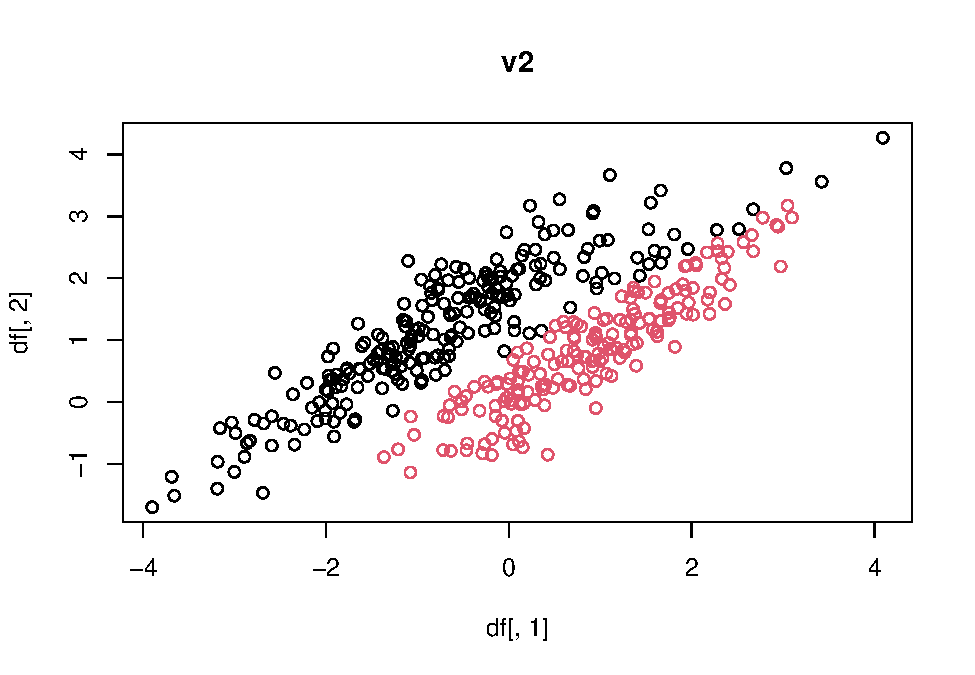
\includegraphics{final_GCM_files/figure-latex/unnamed-chunk-4-1.pdf}

\hypertarget{section-7}{%
\subsection{2.2}\label{section-7}}

\begin{Shaded}
\begin{Highlighting}[]
\DocumentationTok{\#\#\#\#\#\#\#\#\#\#\#\#\#\#\#\#\#\#\#\#\#\#\#\#\#\#\#\#\#}
\CommentTok{\# for(i in 1:7)\{}
\CommentTok{\#   df=data.frame(prob2.list[[i]])}
\CommentTok{\#   mcl.model \textless{}{-} Mclust(df, 2)}
\CommentTok{\#   plot(mcl.model, what = "classification", main = "Mclust Classification")}
\CommentTok{\# \}}


\CommentTok{\# initialk \textless{}{-} mclust::hc(data = df, modelName = "EII")}
\CommentTok{\# initialk \textless{}{-} mclust::hclass(initialk, 2)}
\CommentTok{\# mu \textless{}{-} split(df[, 1:2], initialk)}
\CommentTok{\# mu \textless{}{-} t(sapply(mu, colMeans))}
\CommentTok{\# cov\_mat \textless{}{-} cov(df)\#list(diag(4), diag(4))}
\CommentTok{\# }
\CommentTok{\# \# Mixing Components}
\CommentTok{\# a \textless{}{-} runif(2)}
\CommentTok{\# a \textless{}{-} a/sum(a)}
\CommentTok{\# }
\CommentTok{\# \# Calculate PDF with class means and covariances.}
\CommentTok{\# z \textless{}{-} cbind(mvpdf(x = df, mu = mu[1, ], sigma = cov\_mat), }
\CommentTok{\#            mvpdf(x = df, mu = mu[2, ], sigma = cov\_mat))}
\CommentTok{\# }
\CommentTok{\# \# Expectation Step for each class.}
\CommentTok{\# r \textless{}{-} cbind((a[1] * z[, 1])/rowSums(t((t(z) * a))), }
\CommentTok{\#            (a[2] * z[, 2])/rowSums(t((t(z) * a))))}
\CommentTok{\# }
\CommentTok{\# \# Choose the highest rowwise probability}
\CommentTok{\# eK \textless{}{-} factor(apply(r, 1, which.max))}
\CommentTok{\# }
\CommentTok{\# \# Total Responsibility}
\CommentTok{\# mc \textless{}{-} colSums(r)}
\CommentTok{\# \# Update Mixing Components.}
\CommentTok{\# a \textless{}{-} mc/NROW(df)}
\CommentTok{\# \# Update our Means}
\CommentTok{\# mu \textless{}{-} rbind(colSums(df[, 1:2] * r[, 1]) * 1/mc[1], }
\CommentTok{\#             colSums(df[, 1:2] * r[, 2]) * 1/mc[2])}
\CommentTok{\# \# Update Covariance matrix.}
\CommentTok{\# cov\_mat \textless{}{-} t(r[, 1] * t(apply(df[, 1:2], 1, function(x) x {-} mu[1, ]))) \%*\% }
\CommentTok{\#     (r[, 1] * t(apply(df[, 1:2], 1, function(x) x {-} mu[1, ]))) * 1/mc[1]}
\end{Highlighting}
\end{Shaded}

\hypertarget{section-8}{%
\subsection{2.3}\label{section-8}}

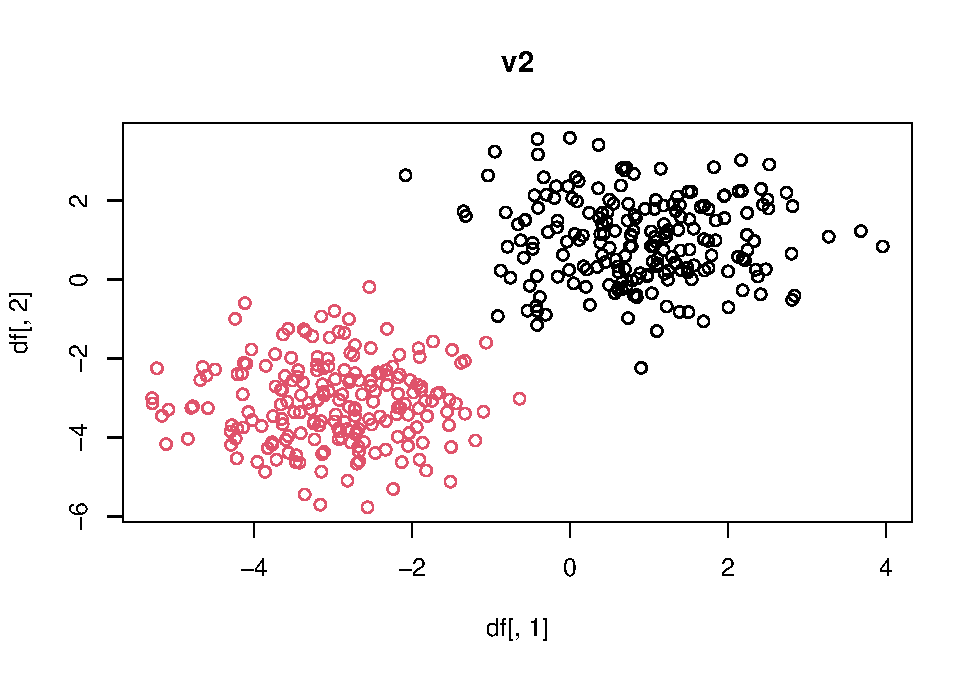
\includegraphics[width=0.33\linewidth]{final_GCM_files/figure-latex/unnamed-chunk-7-1}
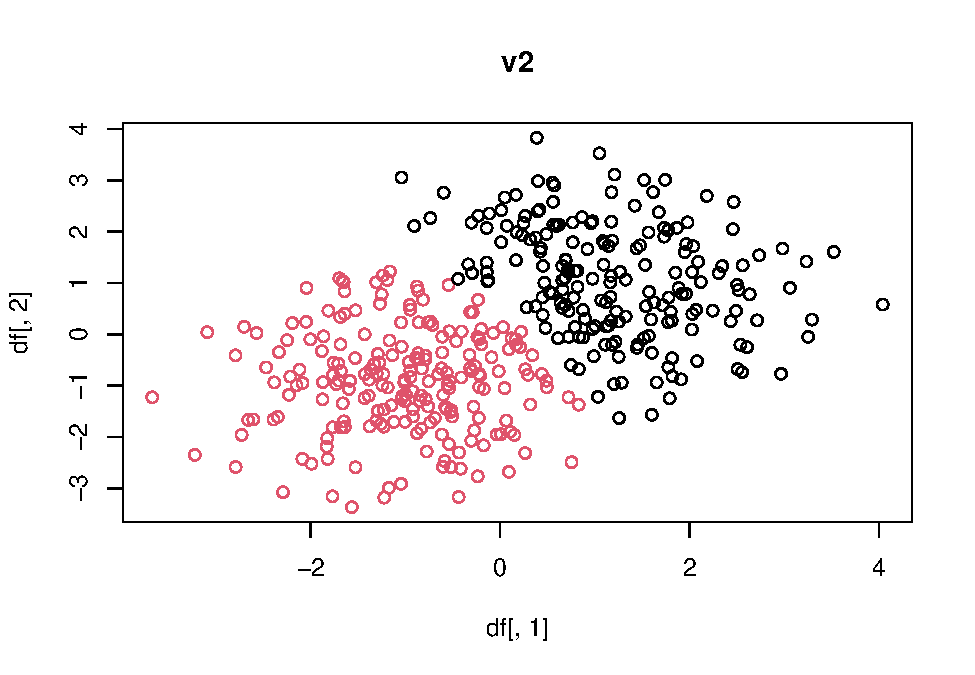
\includegraphics[width=0.33\linewidth]{final_GCM_files/figure-latex/unnamed-chunk-7-2}
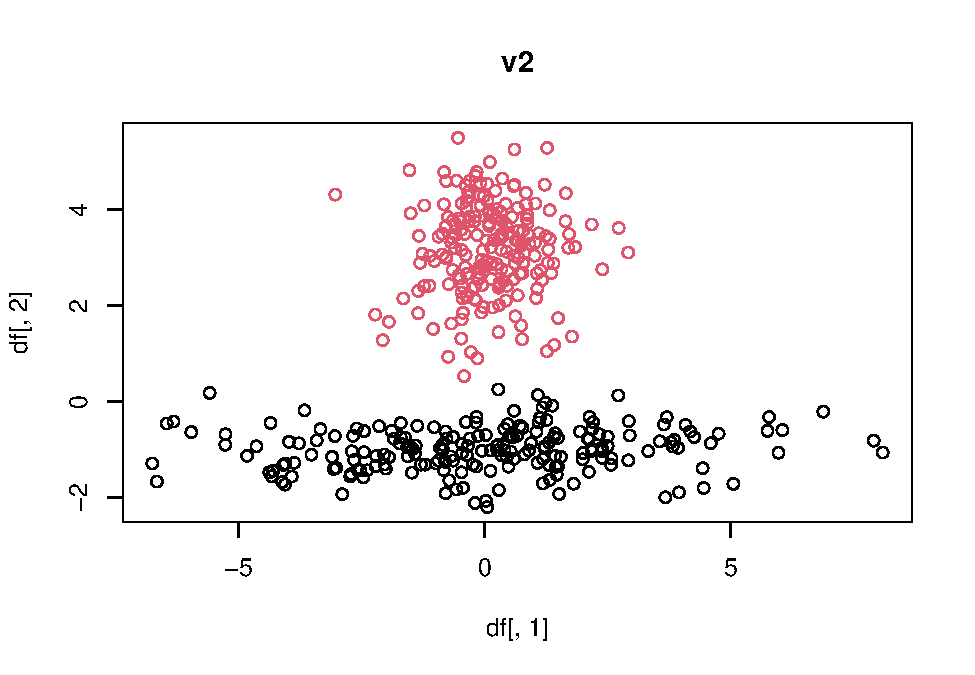
\includegraphics[width=0.33\linewidth]{final_GCM_files/figure-latex/unnamed-chunk-7-3}
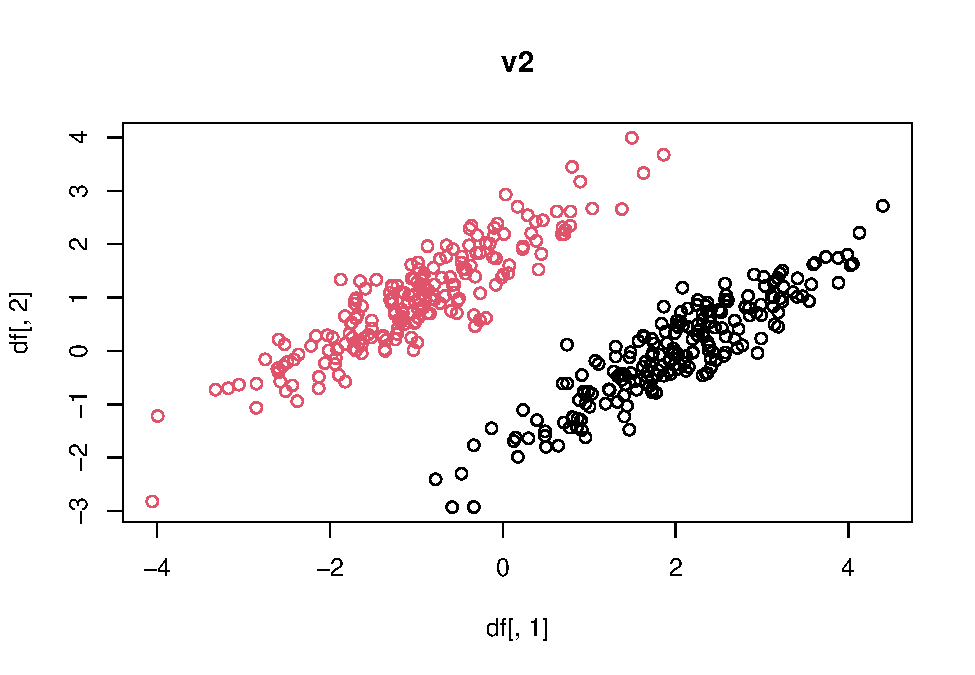
\includegraphics[width=0.33\linewidth]{final_GCM_files/figure-latex/unnamed-chunk-7-4}
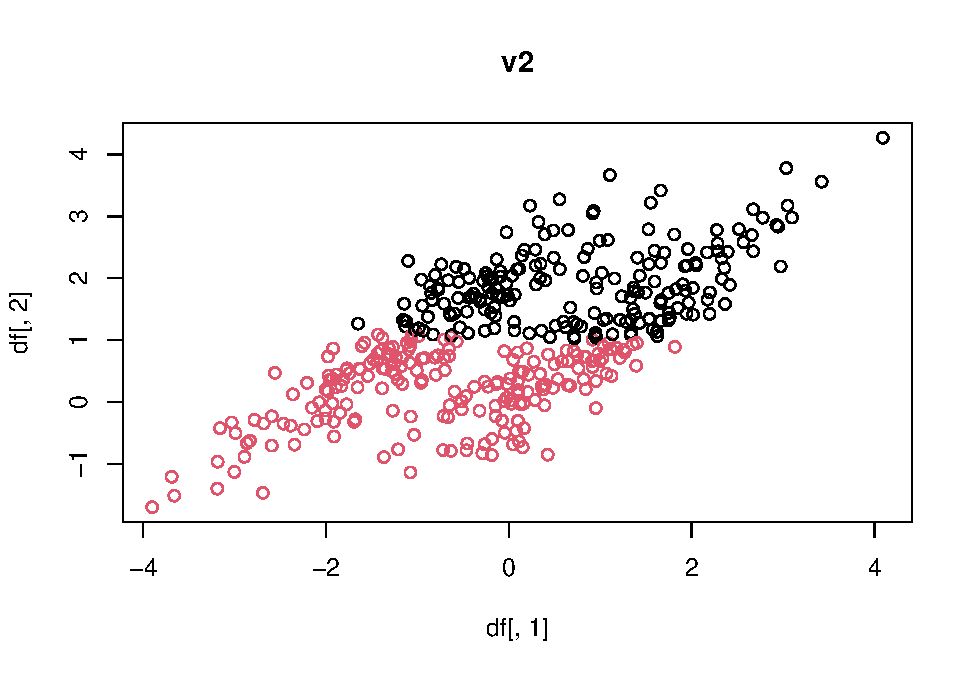
\includegraphics[width=0.33\linewidth]{final_GCM_files/figure-latex/unnamed-chunk-7-5}
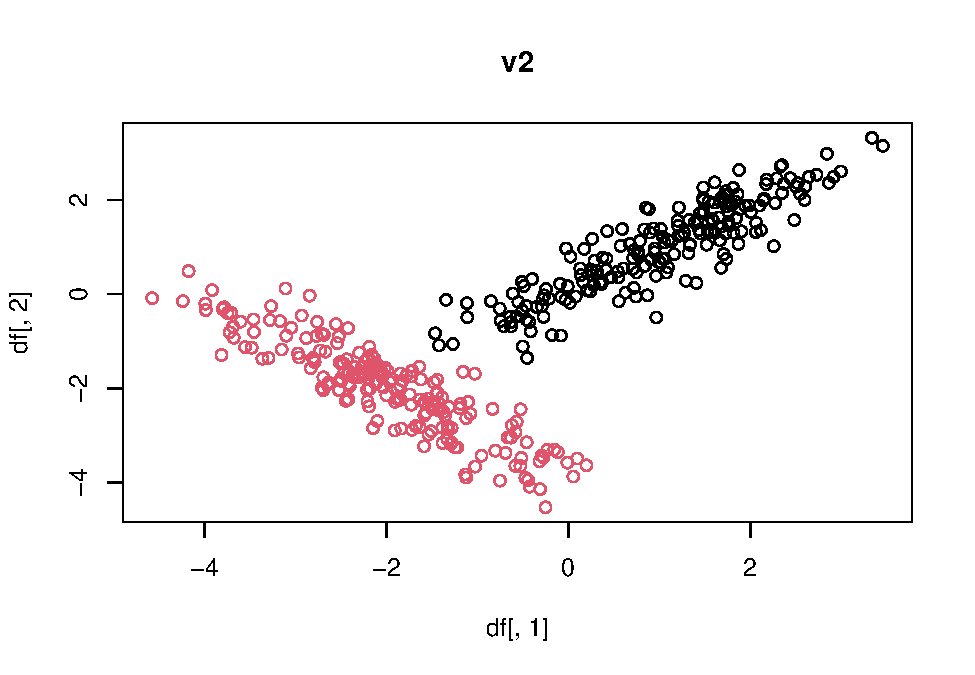
\includegraphics[width=0.33\linewidth]{final_GCM_files/figure-latex/unnamed-chunk-7-6}
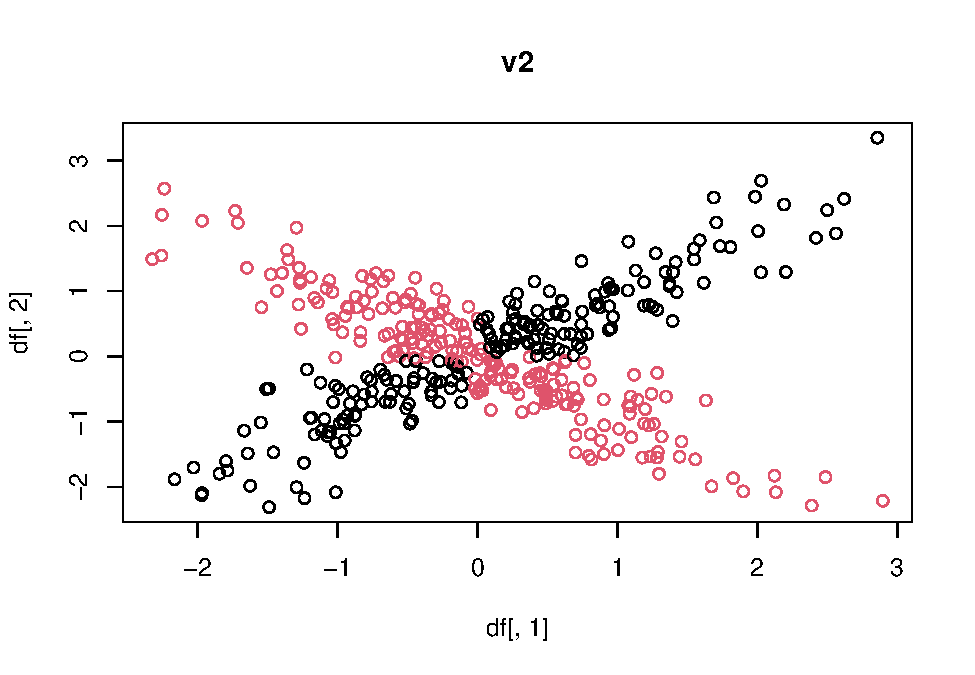
\includegraphics[width=0.33\linewidth]{final_GCM_files/figure-latex/unnamed-chunk-7-7}

\hypertarget{problem-3}{%
\section{Problem 3}\label{problem-3}}

\begin{Shaded}
\begin{Highlighting}[]
\CommentTok{\# initialize information}
\NormalTok{k }\OtherTok{=} \DecValTok{5}
\NormalTok{d\_max }\OtherTok{=} \DecValTok{10}

\CommentTok{\# Mode function}
\NormalTok{Mode }\OtherTok{\textless{}{-}} \ControlFlowTok{function}\NormalTok{(x) \{}
\NormalTok{  ox }\OtherTok{\textless{}{-}} \FunctionTok{order}\NormalTok{(x)}
\NormalTok{  ux }\OtherTok{\textless{}{-}} \FunctionTok{unique}\NormalTok{(ox)}
\NormalTok{  ux[}\FunctionTok{which.max}\NormalTok{(}\FunctionTok{tabulate}\NormalTok{(}\FunctionTok{match}\NormalTok{(x, ux)))]}
\NormalTok{\}}

\CommentTok{\# Outer CV to estimate performance (seed=0)}
\NormalTok{n\_i }\OtherTok{=} \FunctionTok{nrow}\NormalTok{(prob3.df)}
\ControlFlowTok{for}\NormalTok{(k\_i }\ControlFlowTok{in} \FunctionTok{seq}\NormalTok{(k))\{}
\NormalTok{  inds.part }\OtherTok{=} \FunctionTok{myCVids}\NormalTok{(}\AttributeTok{n=}\NormalTok{n\_i, }\AttributeTok{K=}\NormalTok{k, }\AttributeTok{seed=}\DecValTok{0}\NormalTok{)}
\NormalTok{  isk }\OtherTok{=}\NormalTok{ (inds.part }\SpecialCharTok{==}\NormalTok{ k\_i)}
\NormalTok{  valid.i }\OtherTok{=} \FunctionTok{which}\NormalTok{(isk)}
\NormalTok{  train.i }\OtherTok{=} \FunctionTok{which}\NormalTok{(}\SpecialCharTok{!}\NormalTok{isk)}
  \CommentTok{\# split data into train and test sets}
\NormalTok{  data.valid.i }\OtherTok{=}\NormalTok{ prob3.df[valid.i,]}
  \FunctionTok{rownames}\NormalTok{(data.valid.i) }\OtherTok{\textless{}{-}} \ConstantTok{NULL}
\NormalTok{  data.train.i }\OtherTok{=}\NormalTok{ prob3.df[train.i,]}
  \FunctionTok{rownames}\NormalTok{(data.train.i) }\OtherTok{\textless{}{-}} \ConstantTok{NULL}
  
  \CommentTok{\# Inner CV to estimate parameters (seed=1000)}
\NormalTok{  n\_j }\OtherTok{=} \FunctionTok{nrow}\NormalTok{(data.train.i)}
\NormalTok{  d\_opt\_vec }\OtherTok{=} \FunctionTok{c}\NormalTok{()}
\NormalTok{  mse\_opt\_vec }\OtherTok{=} \FunctionTok{c}\NormalTok{()}
  \ControlFlowTok{for}\NormalTok{(k\_j }\ControlFlowTok{in} \FunctionTok{seq}\NormalTok{(k))\{}
\NormalTok{    inds.part }\OtherTok{=} \FunctionTok{myCVids}\NormalTok{(}\AttributeTok{n=}\NormalTok{n\_j, }\AttributeTok{K=}\NormalTok{k, }\AttributeTok{seed=}\DecValTok{1000}\NormalTok{)}
\NormalTok{    isk }\OtherTok{=}\NormalTok{ (inds.part }\SpecialCharTok{==}\NormalTok{ k\_j)}
\NormalTok{    valid.j }\OtherTok{=} \FunctionTok{which}\NormalTok{(isk)}
\NormalTok{    train.j }\OtherTok{=} \FunctionTok{which}\NormalTok{(}\SpecialCharTok{!}\NormalTok{isk)}
    \CommentTok{\# split data into train and test sets}
\NormalTok{    data.valid.j }\OtherTok{=}\NormalTok{ data.train.i[valid.j,]}
\NormalTok{    data.train.j }\OtherTok{=}\NormalTok{ data.train.i[train.j,]}

    \CommentTok{\# test different parameters (d)}
\NormalTok{    lm\_results }\OtherTok{\textless{}{-}} \FunctionTok{lapply}\NormalTok{(}\DecValTok{1}\SpecialCharTok{:}\NormalTok{d\_max, }\ControlFlowTok{function}\NormalTok{(d) }\FunctionTok{lm}\NormalTok{(y }\SpecialCharTok{\textasciitilde{}} \FunctionTok{poly}\NormalTok{(x, d), }\AttributeTok{data =}\NormalTok{ data.train.j))}
\NormalTok{    mse\_vec }\OtherTok{=} \FunctionTok{c}\NormalTok{()}
    \ControlFlowTok{for}\NormalTok{(d }\ControlFlowTok{in} \FunctionTok{seq}\NormalTok{(d\_max))\{}
\NormalTok{      lm.fit.j }\OtherTok{=}\NormalTok{ lm\_results[[d]]}
\NormalTok{      mse\_j }\OtherTok{=} \FunctionTok{mean}\NormalTok{((data.valid.j}\SpecialCharTok{$}\NormalTok{y }\SpecialCharTok{{-}} \FunctionTok{predict}\NormalTok{(lm.fit.j , data.valid.j))}\SpecialCharTok{\^{}}\DecValTok{2}\NormalTok{)}
\NormalTok{      mse\_vec }\OtherTok{=} \FunctionTok{c}\NormalTok{(mse\_vec, mse\_j)}
\NormalTok{    \}}
\NormalTok{    d\_opt }\OtherTok{=} \FunctionTok{which.min}\NormalTok{(mse\_vec)}
\NormalTok{    mse\_opt }\OtherTok{=} \FunctionTok{min}\NormalTok{(mse\_vec)}
\NormalTok{    d\_opt\_vec }\OtherTok{=} \FunctionTok{c}\NormalTok{(d\_opt\_vec, d\_opt)}
\NormalTok{    mse\_opt\_vec }\OtherTok{=} \FunctionTok{c}\NormalTok{(mse\_opt\_vec, mse\_opt)}
    
\NormalTok{    d\_mse\_opt\_df }\OtherTok{=} \FunctionTok{data.frame}\NormalTok{(d\_opt\_vec, mse\_opt\_vec)}
\NormalTok{  \}}
  
  \CommentTok{\# select the mode of parameter d for all inner folds}
  \CommentTok{\# if multiple modes, select the smallest value for d}
\NormalTok{  mode\_d }\OtherTok{=} \FunctionTok{Mode}\NormalTok{(d\_mse\_opt\_df}\SpecialCharTok{$}\NormalTok{d\_opt\_vec)}
  
  \CommentTok{\# use mode\_d to retrain polynomial model on data in outer CV}
\NormalTok{  lm.fit.i }\OtherTok{=} \FunctionTok{lm}\NormalTok{(y }\SpecialCharTok{\textasciitilde{}} \FunctionTok{poly}\NormalTok{(x, mode\_d), }\AttributeTok{data =}\NormalTok{ data.train.i)}
\NormalTok{  mse\_i }\OtherTok{=} \FunctionTok{mean}\NormalTok{((data.valid.i}\SpecialCharTok{$}\NormalTok{y }\SpecialCharTok{{-}} \FunctionTok{predict}\NormalTok{(lm.fit.i , data.valid.i))}\SpecialCharTok{\^{}}\DecValTok{2}\NormalTok{)}
  
  \CommentTok{\# estiamte performance}
  \FunctionTok{print}\NormalTok{(}\FunctionTok{paste}\NormalTok{(mode\_d, mse\_i))}
\NormalTok{\}}
\end{Highlighting}
\end{Shaded}

\begin{verbatim}
## [1] "1 2.22843499520875"
## [1] "1 2.85399744815915"
## [1] "1 3.65318687073941"
## [1] "2 4.12692604883736"
## [1] "2 3.96790085830089"
\end{verbatim}

\begin{Shaded}
\begin{Highlighting}[]
\CommentTok{\# should model be trained in outer and inner loop? yes}
\CommentTok{\# potential drawbacks are computation time}
\CommentTok{\# Report mse and d for outer loop}
\CommentTok{\# report mse and d for inner loop}
\CommentTok{\# group them together print dataframe and then final d and final mse for each outer loop}

\StringTok{"Discuss: potential drawbacks of this approach extended to other ML techniques.}
\StringTok{"}
\end{Highlighting}
\end{Shaded}

\begin{verbatim}
## [1] "Discuss: potential drawbacks of this approach extended to other ML techniques.\n"
\end{verbatim}

\hypertarget{problem-4}{%
\section{Problem 4}\label{problem-4}}

\hypertarget{a}{%
\subsection{4.a}\label{a}}

\begin{Shaded}
\begin{Highlighting}[]
\CommentTok{\# initialize data}
\NormalTok{p }\OtherTok{=} \DecValTok{4}
\NormalTok{k\_max }\OtherTok{=} \DecValTok{5}
\NormalTok{n }\OtherTok{=} \FunctionTok{nrow}\NormalTok{(prob4.df)}
\NormalTok{binM }\OtherTok{=} \FunctionTok{myf}\NormalTok{(p)}
\NormalTok{ids }\OtherTok{=} \FunctionTok{bin2dec}\NormalTok{(binM)}
\NormalTok{ROC\_df }\OtherTok{=} \FunctionTok{data.frame}\NormalTok{(}\FunctionTok{matrix}\NormalTok{(}\AttributeTok{ncol =} \FunctionTok{length}\NormalTok{(ids), }\AttributeTok{nrow =}\NormalTok{ n), }\AttributeTok{Y=}\NormalTok{prob4.df}\SpecialCharTok{$}\NormalTok{Y)}
\FunctionTok{colnames}\NormalTok{(ROC\_df) }\OtherTok{=} \FunctionTok{c}\NormalTok{(ids, }\StringTok{"Y"}\NormalTok{)}

\CommentTok{\# loop through models}
\NormalTok{feature\_names }\OtherTok{=} \FunctionTok{c}\NormalTok{(}\StringTok{"X1"}\NormalTok{,}\StringTok{"X2"}\NormalTok{,}\StringTok{"X3"}\NormalTok{,}\StringTok{"X4"}\NormalTok{)}
\NormalTok{features\_vec }\OtherTok{=} \FunctionTok{c}\NormalTok{()}
\NormalTok{mean\_mcr\_vec }\OtherTok{=} \FunctionTok{c}\NormalTok{()}
\ControlFlowTok{for}\NormalTok{(i }\ControlFlowTok{in} \FunctionTok{seq}\NormalTok{(}\DecValTok{1}\SpecialCharTok{:}\FunctionTok{length}\NormalTok{(ids)))\{}
  
  \CommentTok{\# select subset of data}
\NormalTok{  gamma }\OtherTok{=}\NormalTok{ binM[i,]}
\NormalTok{  alpha }\OtherTok{=}\NormalTok{ ids[i]}
\NormalTok{  X }\OtherTok{=} \FunctionTok{data.frame}\NormalTok{(}\AttributeTok{Intercept=}\DecValTok{1}\NormalTok{, prob4.df[,}\SpecialCharTok{{-}}\DecValTok{5}\NormalTok{][,gamma}\SpecialCharTok{==}\DecValTok{1}\NormalTok{])}
\NormalTok{  Y }\OtherTok{=}\NormalTok{ prob4.df}\SpecialCharTok{$}\NormalTok{Y}
\NormalTok{  data\_df }\OtherTok{=} \FunctionTok{data.frame}\NormalTok{(Y, X)}
  
  \CommentTok{\# get feature names of id}
  \ControlFlowTok{if}\NormalTok{(}\FunctionTok{sum}\NormalTok{(gamma)}\SpecialCharTok{==}\DecValTok{0}\NormalTok{)\{}
\NormalTok{    features }\OtherTok{=} \StringTok{"None"}
\NormalTok{  \}}\ControlFlowTok{else}\NormalTok{\{}
\NormalTok{    features }\OtherTok{=}\NormalTok{ feature\_names[gamma}\SpecialCharTok{==}\DecValTok{1}\NormalTok{]}
\NormalTok{  \}}
\NormalTok{  features\_vec }\OtherTok{=} \FunctionTok{c}\NormalTok{(features\_vec, }\FunctionTok{paste}\NormalTok{(features,}\AttributeTok{collapse=}\StringTok{" "}\NormalTok{))}

  \CommentTok{\# perform 5{-}fold CV}
\NormalTok{  inds.part }\OtherTok{=} \FunctionTok{myCVids}\NormalTok{(n, }\DecValTok{5}\NormalTok{, }\AttributeTok{seed=}\DecValTok{0}\NormalTok{)}
  \CommentTok{\# loop through folds}
\NormalTok{  mcr\_vec }\OtherTok{=} \FunctionTok{c}\NormalTok{()}
  \ControlFlowTok{for}\NormalTok{(k }\ControlFlowTok{in} \FunctionTok{seq}\NormalTok{(}\DecValTok{1}\SpecialCharTok{:}\NormalTok{k\_max))\{}
\NormalTok{    isk }\OtherTok{=}\NormalTok{ (inds.part }\SpecialCharTok{==}\NormalTok{ k)}
\NormalTok{    valid.k }\OtherTok{=} \FunctionTok{which}\NormalTok{(isk)}
\NormalTok{    train.k }\OtherTok{=} \FunctionTok{which}\NormalTok{(}\SpecialCharTok{!}\NormalTok{isk)}

    \CommentTok{\# train logistic regression model}
\NormalTok{    glm.fit }\OtherTok{=} \FunctionTok{glm}\NormalTok{(Y }\SpecialCharTok{\textasciitilde{}} \DecValTok{0} \SpecialCharTok{+}\NormalTok{.,}
                 \AttributeTok{family=}\NormalTok{binomial,}
                 \AttributeTok{data=}\FunctionTok{as.data.frame}\NormalTok{(data\_df[train.k,]))}
    \FunctionTok{print}\NormalTok{(}\FunctionTok{summary}\NormalTok{(glm.fit))}
    
    \CommentTok{\# predict target on validation data  }
\NormalTok{    pred }\OtherTok{=} \FunctionTok{predict}\NormalTok{(glm.fit , data\_df[valid.k,])}
\NormalTok{    ROC\_df[valid.k,i] }\OtherTok{=}\NormalTok{ pred}
    
    \CommentTok{\# calculate mis{-}classification error rate for default 0.5 threshold}
\NormalTok{    mcr }\OtherTok{=} \FunctionTok{MCR}\NormalTok{(}\AttributeTok{target=}\NormalTok{data\_df[valid.k,]}\SpecialCharTok{$}\NormalTok{Y, }\AttributeTok{predicted=}\NormalTok{pred, }\AttributeTok{threshold=}\FloatTok{0.5}\NormalTok{)}
\NormalTok{    mcr\_vec }\OtherTok{=} \FunctionTok{c}\NormalTok{(mcr\_vec, mcr)}
\NormalTok{  \}}
\NormalTok{  mean\_mcr }\OtherTok{=} \FunctionTok{mean}\NormalTok{(mcr\_vec)}
\NormalTok{  mean\_mcr\_vec }\OtherTok{=} \FunctionTok{c}\NormalTok{(mean\_mcr\_vec, mean\_mcr)}
\NormalTok{\}}
\end{Highlighting}
\end{Shaded}

\begin{verbatim}
## 
## Call:
## glm(formula = Y ~ 0 + ., family = binomial, data = as.data.frame(data_df[train.k, 
##     ]))
## 
## Deviance Residuals: 
##    Min      1Q  Median      3Q     Max  
## -1.231  -1.231   1.125   1.125   1.125  
## 
## Coefficients:
##           Estimate Std. Error z value Pr(>|z|)
## Intercept   0.1252     0.1584    0.79    0.429
## 
## (Dispersion parameter for binomial family taken to be 1)
## 
##     Null deviance: 221.81  on 160  degrees of freedom
## Residual deviance: 221.18  on 159  degrees of freedom
## AIC: 223.18
## 
## Number of Fisher Scoring iterations: 3
## 
## 
## Call:
## glm(formula = Y ~ 0 + ., family = binomial, data = as.data.frame(data_df[train.k, 
##     ]))
## 
## Deviance Residuals: 
##    Min      1Q  Median      3Q     Max  
## -1.231  -1.231   1.125   1.125   1.125  
## 
## Coefficients:
##           Estimate Std. Error z value Pr(>|z|)
## Intercept   0.1252     0.1584    0.79    0.429
## 
## (Dispersion parameter for binomial family taken to be 1)
## 
##     Null deviance: 221.81  on 160  degrees of freedom
## Residual deviance: 221.18  on 159  degrees of freedom
## AIC: 223.18
## 
## Number of Fisher Scoring iterations: 3
## 
## 
## Call:
## glm(formula = Y ~ 0 + ., family = binomial, data = as.data.frame(data_df[train.k, 
##     ]))
## 
## Deviance Residuals: 
##    Min      1Q  Median      3Q     Max  
## -1.220  -1.220   1.135   1.135   1.135  
## 
## Coefficients:
##           Estimate Std. Error z value Pr(>|z|)
## Intercept   0.1001     0.1583   0.632    0.527
## 
## (Dispersion parameter for binomial family taken to be 1)
## 
##     Null deviance: 221.81  on 160  degrees of freedom
## Residual deviance: 221.41  on 159  degrees of freedom
## AIC: 223.41
## 
## Number of Fisher Scoring iterations: 3
## 
## 
## Call:
## glm(formula = Y ~ 0 + ., family = binomial, data = as.data.frame(data_df[train.k, 
##     ]))
## 
## Deviance Residuals: 
##    Min      1Q  Median      3Q     Max  
## -1.253  -1.253   1.104   1.104   1.104  
## 
## Coefficients:
##           Estimate Std. Error z value Pr(>|z|)
## Intercept   0.1754     0.1587   1.105    0.269
## 
## (Dispersion parameter for binomial family taken to be 1)
## 
##     Null deviance: 221.81  on 160  degrees of freedom
## Residual deviance: 220.58  on 159  degrees of freedom
## AIC: 222.58
## 
## Number of Fisher Scoring iterations: 3
## 
## 
## Call:
## glm(formula = Y ~ 0 + ., family = binomial, data = as.data.frame(data_df[train.k, 
##     ]))
## 
## Deviance Residuals: 
##    Min      1Q  Median      3Q     Max  
## -1.167  -1.167  -1.167   1.188   1.188  
## 
## Coefficients:
##           Estimate Std. Error z value Pr(>|z|)
## Intercept  -0.0250     0.1581  -0.158    0.874
## 
## (Dispersion parameter for binomial family taken to be 1)
## 
##     Null deviance: 221.81  on 160  degrees of freedom
## Residual deviance: 221.78  on 159  degrees of freedom
## AIC: 223.78
## 
## Number of Fisher Scoring iterations: 3
## 
## 
## Call:
## glm(formula = Y ~ 0 + ., family = binomial, data = as.data.frame(data_df[train.k, 
##     ]))
## 
## Deviance Residuals: 
##    Min      1Q  Median      3Q     Max  
## -1.355  -1.222   1.016   1.127   1.236  
## 
## Coefficients:
##                              Estimate Std. Error z value Pr(>|z|)
## Intercept                      0.1308     0.1591   0.822    0.411
## prob4.df....5....gamma....1.  -0.2845     0.2788  -1.020    0.308
## 
## (Dispersion parameter for binomial family taken to be 1)
## 
##     Null deviance: 221.81  on 160  degrees of freedom
## Residual deviance: 220.13  on 158  degrees of freedom
## AIC: 224.13
## 
## Number of Fisher Scoring iterations: 4
## 
## 
## Call:
## glm(formula = Y ~ 0 + ., family = binomial, data = as.data.frame(data_df[train.k, 
##     ]))
## 
## Deviance Residuals: 
##     Min       1Q   Median       3Q      Max  
## -1.4471  -1.1934   0.9428   1.1244   1.3188  
## 
## Coefficients:
##                              Estimate Std. Error z value Pr(>|z|)  
## Intercept                      0.1355     0.1602   0.846   0.3978  
## prob4.df....5....gamma....1.  -0.4908     0.2763  -1.776   0.0757 .
## ---
## Signif. codes:  0 '***' 0.001 '**' 0.01 '*' 0.05 '.' 0.1 ' ' 1
## 
## (Dispersion parameter for binomial family taken to be 1)
## 
##     Null deviance: 221.81  on 160  degrees of freedom
## Residual deviance: 217.97  on 158  degrees of freedom
## AIC: 221.97
## 
## Number of Fisher Scoring iterations: 4
## 
## 
## Call:
## glm(formula = Y ~ 0 + ., family = binomial, data = as.data.frame(data_df[train.k, 
##     ]))
## 
## Deviance Residuals: 
##     Min       1Q   Median       3Q      Max  
## -1.3858  -1.2121   0.9776   1.1276   1.3067  
## 
## Coefficients:
##                              Estimate Std. Error z value Pr(>|z|)
## Intercept                      0.0986     0.1594   0.619    0.536
## prob4.df....5....gamma....1.  -0.4225     0.2892  -1.461    0.144
## 
## (Dispersion parameter for binomial family taken to be 1)
## 
##     Null deviance: 221.81  on 160  degrees of freedom
## Residual deviance: 219.24  on 158  degrees of freedom
## AIC: 223.24
## 
## Number of Fisher Scoring iterations: 4
## 
## 
## Call:
## glm(formula = Y ~ 0 + ., family = binomial, data = as.data.frame(data_df[train.k, 
##     ]))
## 
## Deviance Residuals: 
##     Min       1Q   Median       3Q      Max  
## -1.6098  -1.1572   0.8224   1.0902   1.3832  
## 
## Coefficients:
##                              Estimate Std. Error z value Pr(>|z|)   
## Intercept                      0.2233     0.1638   1.363  0.17274   
## prob4.df....5....gamma....1.  -0.7708     0.2985  -2.582  0.00982 **
## ---
## Signif. codes:  0 '***' 0.001 '**' 0.01 '*' 0.05 '.' 0.1 ' ' 1
## 
## (Dispersion parameter for binomial family taken to be 1)
## 
##     Null deviance: 221.81  on 160  degrees of freedom
## Residual deviance: 213.61  on 158  degrees of freedom
## AIC: 217.61
## 
## Number of Fisher Scoring iterations: 4
## 
## 
## Call:
## glm(formula = Y ~ 0 + ., family = binomial, data = as.data.frame(data_df[train.k, 
##     ]))
## 
## Deviance Residuals: 
##    Min      1Q  Median      3Q     Max  
## -1.315  -1.165  -1.029   1.177   1.325  
## 
## Coefficients:
##                              Estimate Std. Error z value Pr(>|z|)
## Intercept                    -0.01766    0.15896  -0.111    0.912
## prob4.df....5....gamma....1. -0.34432    0.28669  -1.201    0.230
## 
## (Dispersion parameter for binomial family taken to be 1)
## 
##     Null deviance: 221.81  on 160  degrees of freedom
## Residual deviance: 220.33  on 158  degrees of freedom
## AIC: 224.33
## 
## Number of Fisher Scoring iterations: 3
## 
## 
## Call:
## glm(formula = Y ~ 0 + ., family = binomial, data = as.data.frame(data_df[train.k, 
##     ]))
## 
## Deviance Residuals: 
##     Min       1Q   Median       3Q      Max  
## -1.7517  -1.0733   0.7224   1.0568   1.5349  
## 
## Coefficients:
##                              Estimate Std. Error z value Pr(>|z|)    
## Intercept                      0.2097     0.1681   1.248 0.212206    
## prob4.df....5....gamma....1.  -1.0856     0.3024  -3.590 0.000331 ***
## ---
## Signif. codes:  0 '***' 0.001 '**' 0.01 '*' 0.05 '.' 0.1 ' ' 1
## 
## (Dispersion parameter for binomial family taken to be 1)
## 
##     Null deviance: 221.81  on 160  degrees of freedom
## Residual deviance: 207.09  on 158  degrees of freedom
## AIC: 211.09
## 
## Number of Fisher Scoring iterations: 4
## 
## 
## Call:
## glm(formula = Y ~ 0 + ., family = binomial, data = as.data.frame(data_df[train.k, 
##     ]))
## 
## Deviance Residuals: 
##     Min       1Q   Median       3Q      Max  
## -1.7626  -1.0585   0.7138   1.0415   1.5710  
## 
## Coefficients:
##                              Estimate Std. Error z value Pr(>|z|)    
## Intercept                      0.1803     0.1677   1.075 0.282279    
## prob4.df....5....gamma....1.  -1.1396     0.3013  -3.782 0.000156 ***
## ---
## Signif. codes:  0 '***' 0.001 '**' 0.01 '*' 0.05 '.' 0.1 ' ' 1
## 
## (Dispersion parameter for binomial family taken to be 1)
## 
##     Null deviance: 221.81  on 160  degrees of freedom
## Residual deviance: 205.38  on 158  degrees of freedom
## AIC: 209.38
## 
## Number of Fisher Scoring iterations: 4
## 
## 
## Call:
## glm(formula = Y ~ 0 + ., family = binomial, data = as.data.frame(data_df[train.k, 
##     ]))
## 
## Deviance Residuals: 
##     Min       1Q   Median       3Q      Max  
## -1.6445  -1.1025   0.7911   1.0539   1.5266  
## 
## Coefficients:
##                              Estimate Std. Error z value Pr(>|z|)    
## Intercept                      0.1034     0.1645   0.628 0.529698    
## prob4.df....5....gamma....1.  -0.9531     0.2838  -3.358 0.000785 ***
## ---
## Signif. codes:  0 '***' 0.001 '**' 0.01 '*' 0.05 '.' 0.1 ' ' 1
## 
## (Dispersion parameter for binomial family taken to be 1)
## 
##     Null deviance: 221.81  on 160  degrees of freedom
## Residual deviance: 209.32  on 158  degrees of freedom
## AIC: 213.32
## 
## Number of Fisher Scoring iterations: 4
## 
## 
## Call:
## glm(formula = Y ~ 0 + ., family = binomial, data = as.data.frame(data_df[train.k, 
##     ]))
## 
## Deviance Residuals: 
##     Min       1Q   Median       3Q      Max  
## -1.7537  -1.0814   0.7114   1.0311   1.5433  
## 
## Coefficients:
##                              Estimate Std. Error z value Pr(>|z|)    
## Intercept                      0.2325     0.1681   1.383 0.166696    
## prob4.df....5....gamma....1.  -1.1298     0.3000  -3.766 0.000166 ***
## ---
## Signif. codes:  0 '***' 0.001 '**' 0.01 '*' 0.05 '.' 0.1 ' ' 1
## 
## (Dispersion parameter for binomial family taken to be 1)
## 
##     Null deviance: 221.81  on 160  degrees of freedom
## Residual deviance: 204.96  on 158  degrees of freedom
## AIC: 208.96
## 
## Number of Fisher Scoring iterations: 4
## 
## 
## Call:
## glm(formula = Y ~ 0 + ., family = binomial, data = as.data.frame(data_df[train.k, 
##     ]))
## 
## Deviance Residuals: 
##    Min      1Q  Median      3Q     Max  
## -1.680  -1.050  -0.771   1.082   1.602  
## 
## Coefficients:
##                              Estimate Std. Error z value Pr(>|z|)    
## Intercept                     0.03143    0.16671   0.189 0.850444    
## prob4.df....5....gamma....1. -1.10361    0.29682  -3.718 0.000201 ***
## ---
## Signif. codes:  0 '***' 0.001 '**' 0.01 '*' 0.05 '.' 0.1 ' ' 1
## 
## (Dispersion parameter for binomial family taken to be 1)
## 
##     Null deviance: 221.81  on 160  degrees of freedom
## Residual deviance: 206.63  on 158  degrees of freedom
## AIC: 210.63
## 
## Number of Fisher Scoring iterations: 4
## 
## 
## Call:
## glm(formula = Y ~ 0 + ., family = binomial, data = as.data.frame(data_df[train.k, 
##     ]))
## 
## Deviance Residuals: 
##    Min      1Q  Median      3Q     Max  
## -1.766  -1.059   0.717   1.066   1.556  
## 
## Coefficients:
##           Estimate Std. Error z value Pr(>|z|)    
## Intercept   0.2142     0.1686   1.271 0.203846    
## X3         -1.0761     0.3029  -3.552 0.000382 ***
## X4         -0.2453     0.2903  -0.845 0.398144    
## ---
## Signif. codes:  0 '***' 0.001 '**' 0.01 '*' 0.05 '.' 0.1 ' ' 1
## 
## (Dispersion parameter for binomial family taken to be 1)
## 
##     Null deviance: 221.81  on 160  degrees of freedom
## Residual deviance: 206.37  on 157  degrees of freedom
## AIC: 212.37
## 
## Number of Fisher Scoring iterations: 4
## 
## 
## Call:
## glm(formula = Y ~ 0 + ., family = binomial, data = as.data.frame(data_df[train.k, 
##     ]))
## 
## Deviance Residuals: 
##     Min       1Q   Median       3Q      Max  
## -1.8861  -1.0387   0.6831   1.0717   1.6278  
## 
## Coefficients:
##           Estimate Std. Error z value Pr(>|z|)    
## Intercept   0.1907     0.1693   1.126 0.260073    
## X3         -1.1246     0.3035  -3.706 0.000211 ***
## X4         -0.4548     0.2890  -1.573 0.115637    
## ---
## Signif. codes:  0 '***' 0.001 '**' 0.01 '*' 0.05 '.' 0.1 ' ' 1
## 
## (Dispersion parameter for binomial family taken to be 1)
## 
##     Null deviance: 221.81  on 160  degrees of freedom
## Residual deviance: 202.87  on 157  degrees of freedom
## AIC: 208.87
## 
## Number of Fisher Scoring iterations: 4
## 
## 
## Call:
## glm(formula = Y ~ 0 + ., family = binomial, data = as.data.frame(data_df[train.k, 
##     ]))
## 
## Deviance Residuals: 
##     Min       1Q   Median       3Q      Max  
## -1.7360  -1.0664   0.7653   1.0749   1.5719  
## 
## Coefficients:
##           Estimate Std. Error z value Pr(>|z|)   
## Intercept   0.1016     0.1653   0.615  0.53881   
## X3         -0.9332     0.2850  -3.274  0.00106 **
## X4         -0.3662     0.2985  -1.227  0.21993   
## ---
## Signif. codes:  0 '***' 0.001 '**' 0.01 '*' 0.05 '.' 0.1 ' ' 1
## 
## (Dispersion parameter for binomial family taken to be 1)
## 
##     Null deviance: 221.81  on 160  degrees of freedom
## Residual deviance: 207.81  on 157  degrees of freedom
## AIC: 213.81
## 
## Number of Fisher Scoring iterations: 4
## 
## 
## Call:
## glm(formula = Y ~ 0 + ., family = binomial, data = as.data.frame(data_df[train.k, 
##     ]))
## 
## Deviance Residuals: 
##     Min       1Q   Median       3Q      Max  
## -2.0198  -1.0431   0.6322   1.0412   1.6317  
## 
## Coefficients:
##           Estimate Std. Error z value Pr(>|z|)    
## Intercept   0.2774     0.1728   1.605 0.108439    
## X3         -1.1062     0.3053  -3.623 0.000291 ***
## X4         -0.7266     0.3089  -2.353 0.018645 *  
## ---
## Signif. codes:  0 '***' 0.001 '**' 0.01 '*' 0.05 '.' 0.1 ' ' 1
## 
## (Dispersion parameter for binomial family taken to be 1)
## 
##     Null deviance: 221.81  on 160  degrees of freedom
## Residual deviance: 199.25  on 157  degrees of freedom
## AIC: 205.25
## 
## Number of Fisher Scoring iterations: 4
## 
## 
## Call:
## glm(formula = Y ~ 0 + ., family = binomial, data = as.data.frame(data_df[train.k, 
##     ]))
## 
## Deviance Residuals: 
##     Min       1Q   Median       3Q      Max  
## -1.7355  -1.0157  -0.7132   1.1123   1.6477  
## 
## Coefficients:
##           Estimate Std. Error z value Pr(>|z|)    
## Intercept  0.03625    0.16724   0.217 0.828387    
## X3        -1.08778    0.29764  -3.655 0.000257 ***
## X4        -0.28116    0.30016  -0.937 0.348912    
## ---
## Signif. codes:  0 '***' 0.001 '**' 0.01 '*' 0.05 '.' 0.1 ' ' 1
## 
## (Dispersion parameter for binomial family taken to be 1)
## 
##     Null deviance: 221.81  on 160  degrees of freedom
## Residual deviance: 205.75  on 157  degrees of freedom
## AIC: 211.75
## 
## Number of Fisher Scoring iterations: 4
## 
## 
## Call:
## glm(formula = Y ~ 0 + ., family = binomial, data = as.data.frame(data_df[train.k, 
##     ]))
## 
## Deviance Residuals: 
##    Min      1Q  Median      3Q     Max  
## -1.238  -1.230   1.118   1.126   1.130  
## 
## Coefficients:
##                              Estimate Std. Error z value Pr(>|z|)
## Intercept                     0.12616    0.15944   0.791    0.429
## prob4.df....5....gamma....1.  0.01553    0.27890   0.056    0.956
## 
## (Dispersion parameter for binomial family taken to be 1)
## 
##     Null deviance: 221.81  on 160  degrees of freedom
## Residual deviance: 221.18  on 158  degrees of freedom
## AIC: 225.18
## 
## Number of Fisher Scoring iterations: 3
## 
## 
## Call:
## glm(formula = Y ~ 0 + ., family = binomial, data = as.data.frame(data_df[train.k, 
##     ]))
## 
## Deviance Residuals: 
##     Min       1Q   Median       3Q      Max  
## -1.4016  -1.1966   0.9796   1.1368   1.2565  
## 
## Coefficients:
##                              Estimate Std. Error z value Pr(>|z|)
## Intercept                      0.1509     0.1607   0.939    0.348
## prob4.df....5....gamma....1.   0.3724     0.2860   1.302    0.193
## 
## (Dispersion parameter for binomial family taken to be 1)
## 
##     Null deviance: 221.81  on 160  degrees of freedom
## Residual deviance: 219.47  on 158  degrees of freedom
## AIC: 223.47
## 
## Number of Fisher Scoring iterations: 4
## 
## 
## Call:
## glm(formula = Y ~ 0 + ., family = binomial, data = as.data.frame(data_df[train.k, 
##     ]))
## 
## Deviance Residuals: 
##    Min      1Q  Median      3Q     Max  
## -1.225  -1.220   1.130   1.135   1.141  
## 
## Coefficients:
##                              Estimate Std. Error z value Pr(>|z|)
## Intercept                     0.09977    0.15843   0.630    0.529
## prob4.df....5....gamma....1. -0.01403    0.27363  -0.051    0.959
## 
## (Dispersion parameter for binomial family taken to be 1)
## 
##     Null deviance: 221.81  on 160  degrees of freedom
## Residual deviance: 221.40  on 158  degrees of freedom
## AIC: 225.4
## 
## Number of Fisher Scoring iterations: 3
## 
## 
## Call:
## glm(formula = Y ~ 0 + ., family = binomial, data = as.data.frame(data_df[train.k, 
##     ]))
## 
## Deviance Residuals: 
##    Min      1Q  Median      3Q     Max  
## -1.303  -1.242   1.061   1.110   1.145  
## 
## Coefficients:
##                              Estimate Std. Error z value Pr(>|z|)
## Intercept                      0.1793     0.1591   1.127    0.260
## prob4.df....5....gamma....1.   0.1143     0.2789   0.410    0.682
## 
## (Dispersion parameter for binomial family taken to be 1)
## 
##     Null deviance: 221.81  on 160  degrees of freedom
## Residual deviance: 220.41  on 158  degrees of freedom
## AIC: 224.41
## 
## Number of Fisher Scoring iterations: 3
## 
## 
## Call:
## glm(formula = Y ~ 0 + ., family = binomial, data = as.data.frame(data_df[train.k, 
##     ]))
## 
## Deviance Residuals: 
##    Min      1Q  Median      3Q     Max  
## -1.388  -1.133  -1.004   1.182   1.357  
## 
## Coefficients:
##                              Estimate Std. Error z value Pr(>|z|)  
## Intercept                     0.01904    0.16178   0.118   0.9063  
## prob4.df....5....gamma....1.  0.47649    0.28382   1.679   0.0932 .
## ---
## Signif. codes:  0 '***' 0.001 '**' 0.01 '*' 0.05 '.' 0.1 ' ' 1
## 
## (Dispersion parameter for binomial family taken to be 1)
## 
##     Null deviance: 221.81  on 160  degrees of freedom
## Residual deviance: 218.91  on 158  degrees of freedom
## AIC: 222.91
## 
## Number of Fisher Scoring iterations: 4
## 
## 
## Call:
## glm(formula = Y ~ 0 + ., family = binomial, data = as.data.frame(data_df[train.k, 
##     ]))
## 
## Deviance Residuals: 
##    Min      1Q  Median      3Q     Max  
## -1.352  -1.221   1.015   1.128   1.240  
## 
## Coefficients:
##            Estimate Std. Error z value Pr(>|z|)
## Intercept  0.131426   0.160068   0.821    0.412
## X2         0.009826   0.279857   0.035    0.972
## X4        -0.284262   0.278881  -1.019    0.308
## 
## (Dispersion parameter for binomial family taken to be 1)
## 
##     Null deviance: 221.81  on 160  degrees of freedom
## Residual deviance: 220.13  on 157  degrees of freedom
## AIC: 226.13
## 
## Number of Fisher Scoring iterations: 4
## 
## 
## Call:
## glm(formula = Y ~ 0 + ., family = binomial, data = as.data.frame(data_df[train.k, 
##     ]))
## 
## Deviance Residuals: 
##     Min       1Q   Median       3Q      Max  
## -1.5269  -1.1775   0.8706   1.1022   1.4541  
## 
## Coefficients:
##           Estimate Std. Error z value Pr(>|z|)  
## Intercept   0.1608     0.1624   0.990   0.3221  
## X2          0.3686     0.2888   1.276   0.2018  
## X4         -0.4886     0.2780  -1.758   0.0788 .
## ---
## Signif. codes:  0 '***' 0.001 '**' 0.01 '*' 0.05 '.' 0.1 ' ' 1
## 
## (Dispersion parameter for binomial family taken to be 1)
## 
##     Null deviance: 221.81  on 160  degrees of freedom
## Residual deviance: 216.32  on 157  degrees of freedom
## AIC: 222.32
## 
## Number of Fisher Scoring iterations: 4
## 
## 
## Call:
## glm(formula = Y ~ 0 + ., family = binomial, data = as.data.frame(data_df[train.k, 
##     ]))
## 
## Deviance Residuals: 
##     Min       1Q   Median       3Q      Max  
## -1.3865  -1.2166   0.9784   1.1325   1.3046  
## 
## Coefficients:
##           Estimate Std. Error z value Pr(>|z|)
## Intercept  0.09811    0.15952   0.615    0.539
## X2        -0.02082    0.27566  -0.076    0.940
## X4        -0.42290    0.28927  -1.462    0.144
## 
## (Dispersion parameter for binomial family taken to be 1)
## 
##     Null deviance: 221.81  on 160  degrees of freedom
## Residual deviance: 219.24  on 157  degrees of freedom
## AIC: 225.24
## 
## Number of Fisher Scoring iterations: 4
## 
## 
## Call:
## glm(formula = Y ~ 0 + ., family = binomial, data = as.data.frame(data_df[train.k, 
##     ]))
## 
## Deviance Residuals: 
##     Min       1Q   Median       3Q      Max  
## -1.5819  -1.1586   0.8254   1.1000   1.4070  
## 
## Coefficients:
##           Estimate Std. Error z value Pr(>|z|)  
## Intercept  0.22595    0.16411   1.377   0.1685  
## X2         0.08317    0.28563   0.291   0.7709  
## X4        -0.76731    0.29886  -2.567   0.0102 *
## ---
## Signif. codes:  0 '***' 0.001 '**' 0.01 '*' 0.05 '.' 0.1 ' ' 1
## 
## (Dispersion parameter for binomial family taken to be 1)
## 
##     Null deviance: 221.81  on 160  degrees of freedom
## Residual deviance: 213.52  on 157  degrees of freedom
## AIC: 219.52
## 
## Number of Fisher Scoring iterations: 4
## 
## 
## Call:
## glm(formula = Y ~ 0 + ., family = binomial, data = as.data.frame(data_df[train.k, 
##     ]))
## 
## Deviance Residuals: 
##     Min       1Q   Median       3Q      Max  
## -1.4365  -1.1356  -0.9306   1.1704   1.4758  
## 
## Coefficients:
##           Estimate Std. Error z value Pr(>|z|)
## Intercept  0.02332    0.16235   0.144    0.886
## X2         0.45449    0.28510   1.594    0.111
## X4        -0.31175    0.28980  -1.076    0.282
## 
## (Dispersion parameter for binomial family taken to be 1)
## 
##     Null deviance: 221.81  on 160  degrees of freedom
## Residual deviance: 217.75  on 157  degrees of freedom
## AIC: 223.75
## 
## Number of Fisher Scoring iterations: 4
## 
## 
## Call:
## glm(formula = Y ~ 0 + ., family = binomial, data = as.data.frame(data_df[train.k, 
##     ]))
## 
## Deviance Residuals: 
##     Min       1Q   Median       3Q      Max  
## -1.7708  -1.0843   0.7259   1.0603   1.5652  
## 
## Coefficients:
##           Estimate Std. Error z value Pr(>|z|)    
## Intercept  0.20605    0.16896   1.219 0.222664    
## X2        -0.06058    0.29195  -0.207 0.835619    
## X3        -1.09009    0.30332  -3.594 0.000326 ***
## ---
## Signif. codes:  0 '***' 0.001 '**' 0.01 '*' 0.05 '.' 0.1 ' ' 1
## 
## (Dispersion parameter for binomial family taken to be 1)
## 
##     Null deviance: 221.81  on 160  degrees of freedom
## Residual deviance: 207.05  on 157  degrees of freedom
## AIC: 213.05
## 
## Number of Fisher Scoring iterations: 4
## 
## 
## Call:
## glm(formula = Y ~ 0 + ., family = binomial, data = as.data.frame(data_df[train.k, 
##     ]))
## 
## Deviance Residuals: 
##     Min       1Q   Median       3Q      Max  
## -1.8104  -1.0569   0.6322   1.0504   1.6650  
## 
## Coefficients:
##           Estimate Std. Error z value Pr(>|z|)    
## Intercept   0.2087     0.1702   1.226 0.220060    
## X2          0.4030     0.3023   1.333 0.182404    
## X3         -1.1499     0.3034  -3.790 0.000151 ***
## ---
## Signif. codes:  0 '***' 0.001 '**' 0.01 '*' 0.05 '.' 0.1 ' ' 1
## 
## (Dispersion parameter for binomial family taken to be 1)
## 
##     Null deviance: 221.81  on 160  degrees of freedom
## Residual deviance: 203.57  on 157  degrees of freedom
## AIC: 209.57
## 
## Number of Fisher Scoring iterations: 4
## 
## 
## Call:
## glm(formula = Y ~ 0 + ., family = binomial, data = as.data.frame(data_df[train.k, 
##     ]))
## 
## Deviance Residuals: 
##     Min       1Q   Median       3Q      Max  
## -1.6437  -1.1023   0.7909   1.0541   1.5253  
## 
## Coefficients:
##            Estimate Std. Error z value Pr(>|z|)    
## Intercept  0.103473   0.164662   0.628 0.529744    
## X2         0.003014   0.284470   0.011 0.991546    
## X3        -0.953145   0.283881  -3.358 0.000786 ***
## ---
## Signif. codes:  0 '***' 0.001 '**' 0.01 '*' 0.05 '.' 0.1 ' ' 1
## 
## (Dispersion parameter for binomial family taken to be 1)
## 
##     Null deviance: 221.81  on 160  degrees of freedom
## Residual deviance: 209.32  on 157  degrees of freedom
## AIC: 215.32
## 
## Number of Fisher Scoring iterations: 4
## 
## 
## Call:
## glm(formula = Y ~ 0 + ., family = binomial, data = as.data.frame(data_df[train.k, 
##     ]))
## 
## Deviance Residuals: 
##     Min       1Q   Median       3Q      Max  
## -1.7452  -1.0747   0.7092   1.0336   1.5250  
## 
## Coefficients:
##           Estimate Std. Error z value Pr(>|z|)    
## Intercept  0.23389    0.16840   1.389 0.164882    
## X2         0.04334    0.29312   0.148 0.882441    
## X3        -1.12703    0.30056  -3.750 0.000177 ***
## ---
## Signif. codes:  0 '***' 0.001 '**' 0.01 '*' 0.05 '.' 0.1 ' ' 1
## 
## (Dispersion parameter for binomial family taken to be 1)
## 
##     Null deviance: 221.81  on 160  degrees of freedom
## Residual deviance: 204.94  on 157  degrees of freedom
## AIC: 210.94
## 
## Number of Fisher Scoring iterations: 4
## 
## 
## Call:
## glm(formula = Y ~ 0 + ., family = binomial, data = as.data.frame(data_df[train.k, 
##     ]))
## 
## Deviance Residuals: 
##     Min       1Q   Median       3Q      Max  
## -1.6675  -1.0704  -0.6972   1.0539   1.6640  
## 
## Coefficients:
##           Estimate Std. Error z value Pr(>|z|)    
## Intercept  0.07322    0.17028   0.430 0.667185    
## X2         0.45739    0.29869   1.531 0.125685    
## X3        -1.09471    0.29880  -3.664 0.000249 ***
## ---
## Signif. codes:  0 '***' 0.001 '**' 0.01 '*' 0.05 '.' 0.1 ' ' 1
## 
## (Dispersion parameter for binomial family taken to be 1)
## 
##     Null deviance: 221.81  on 160  degrees of freedom
## Residual deviance: 204.25  on 157  degrees of freedom
## AIC: 210.25
## 
## Number of Fisher Scoring iterations: 4
## 
## 
## Call:
## glm(formula = Y ~ 0 + ., family = binomial, data = as.data.frame(data_df[train.k, 
##     ]))
## 
## Deviance Residuals: 
##     Min       1Q   Median       3Q      Max  
## -1.7859  -1.0669   0.7184   1.0760   1.5632  
## 
## Coefficients:
##           Estimate Std. Error z value Pr(>|z|)    
## Intercept  0.21052    0.16945   1.242 0.214099    
## X2        -0.06422    0.29247  -0.220 0.826200    
## X3        -1.08060    0.30374  -3.558 0.000374 ***
## X4        -0.24633    0.29051  -0.848 0.396471    
## ---
## Signif. codes:  0 '***' 0.001 '**' 0.01 '*' 0.05 '.' 0.1 ' ' 1
## 
## (Dispersion parameter for binomial family taken to be 1)
## 
##     Null deviance: 221.81  on 160  degrees of freedom
## Residual deviance: 206.33  on 156  degrees of freedom
## AIC: 214.33
## 
## Number of Fisher Scoring iterations: 4
## 
## 
## Call:
## glm(formula = Y ~ 0 + ., family = binomial, data = as.data.frame(data_df[train.k, 
##     ]))
## 
## Deviance Residuals: 
##    Min      1Q  Median      3Q     Max  
## -1.920  -1.063   0.639   1.080   1.778  
## 
## Coefficients:
##           Estimate Std. Error z value Pr(>|z|)    
## Intercept   0.2176     0.1716   1.268 0.204961    
## X2          0.3987     0.3050   1.307 0.191159    
## X3         -1.1353     0.3058  -3.713 0.000205 ***
## X4         -0.4503     0.2903  -1.551 0.120826    
## ---
## Signif. codes:  0 '***' 0.001 '**' 0.01 '*' 0.05 '.' 0.1 ' ' 1
## 
## (Dispersion parameter for binomial family taken to be 1)
## 
##     Null deviance: 221.81  on 160  degrees of freedom
## Residual deviance: 201.14  on 156  degrees of freedom
## AIC: 209.14
## 
## Number of Fisher Scoring iterations: 4
## 
## 
## Call:
## glm(formula = Y ~ 0 + ., family = binomial, data = as.data.frame(data_df[train.k, 
##     ]))
## 
## Deviance Residuals: 
##    Min      1Q  Median      3Q     Max  
## -1.736  -1.066   0.765   1.076   1.572  
## 
## Coefficients:
##            Estimate Std. Error z value Pr(>|z|)   
## Intercept  0.101549   0.165450   0.614  0.53936   
## X2        -0.002754   0.285826  -0.010  0.99231   
## X3        -0.933170   0.285111  -3.273  0.00106 **
## X4        -0.366289   0.298615  -1.227  0.21996   
## ---
## Signif. codes:  0 '***' 0.001 '**' 0.01 '*' 0.05 '.' 0.1 ' ' 1
## 
## (Dispersion parameter for binomial family taken to be 1)
## 
##     Null deviance: 221.81  on 160  degrees of freedom
## Residual deviance: 207.81  on 156  degrees of freedom
## AIC: 215.81
## 
## Number of Fisher Scoring iterations: 4
## 
## 
## Call:
## glm(formula = Y ~ 0 + ., family = binomial, data = as.data.frame(data_df[train.k, 
##     ]))
## 
## Deviance Residuals: 
##     Min       1Q   Median       3Q      Max  
## -2.0200  -1.0432   0.6322   1.0394   1.6307  
## 
## Coefficients:
##            Estimate Std. Error z value Pr(>|z|)    
## Intercept  0.277737   0.173096   1.605 0.108598    
## X2         0.009499   0.300301   0.032 0.974765    
## X3        -1.105577   0.305924  -3.614 0.000302 ***
## X4        -0.726094   0.309318  -2.347 0.018905 *  
## ---
## Signif. codes:  0 '***' 0.001 '**' 0.01 '*' 0.05 '.' 0.1 ' ' 1
## 
## (Dispersion parameter for binomial family taken to be 1)
## 
##     Null deviance: 221.81  on 160  degrees of freedom
## Residual deviance: 199.25  on 156  degrees of freedom
## AIC: 207.25
## 
## Number of Fisher Scoring iterations: 4
## 
## 
## Call:
## glm(formula = Y ~ 0 + ., family = binomial, data = as.data.frame(data_df[train.k, 
##     ]))
## 
## Deviance Residuals: 
##     Min       1Q   Median       3Q      Max  
## -1.7562  -1.0757  -0.6681   1.0543   1.7535  
## 
## Coefficients:
##           Estimate Std. Error z value Pr(>|z|)    
## Intercept  0.07438    0.17049   0.436 0.662620    
## X2         0.43690    0.29985   1.457 0.145097    
## X3        -1.07945    0.29944  -3.605 0.000312 ***
## X4        -0.24373    0.30253  -0.806 0.420450    
## ---
## Signif. codes:  0 '***' 0.001 '**' 0.01 '*' 0.05 '.' 0.1 ' ' 1
## 
## (Dispersion parameter for binomial family taken to be 1)
## 
##     Null deviance: 221.81  on 160  degrees of freedom
## Residual deviance: 203.60  on 156  degrees of freedom
## AIC: 211.6
## 
## Number of Fisher Scoring iterations: 4
## 
## 
## Call:
## glm(formula = Y ~ 0 + ., family = binomial, data = as.data.frame(data_df[train.k, 
##     ]))
## 
## Deviance Residuals: 
##     Min       1Q   Median       3Q      Max  
## -1.5805  -1.1450   0.8609   1.0604   1.4873  
## 
## Coefficients:
##                              Estimate Std. Error z value Pr(>|z|)   
## Intercept                     0.09893    0.16244   0.609  0.54248   
## prob4.df....5....gamma....1.  0.82540    0.30708   2.688  0.00719 **
## ---
## Signif. codes:  0 '***' 0.001 '**' 0.01 '*' 0.05 '.' 0.1 ' ' 1
## 
## (Dispersion parameter for binomial family taken to be 1)
## 
##     Null deviance: 221.81  on 160  degrees of freedom
## Residual deviance: 213.63  on 158  degrees of freedom
## AIC: 217.63
## 
## Number of Fisher Scoring iterations: 4
## 
## 
## Call:
## glm(formula = Y ~ 0 + ., family = binomial, data = as.data.frame(data_df[train.k, 
##     ]))
## 
## Deviance Residuals: 
##     Min       1Q   Median       3Q      Max  
## -1.4536  -1.2090   0.9497   1.1075   1.3484  
## 
## Coefficients:
##                              Estimate Std. Error z value Pr(>|z|)  
## Intercept                      0.1151     0.1600   0.719   0.4719  
## prob4.df....5....gamma....1.   0.5227     0.2987   1.750   0.0802 .
## ---
## Signif. codes:  0 '***' 0.001 '**' 0.01 '*' 0.05 '.' 0.1 ' ' 1
## 
## (Dispersion parameter for binomial family taken to be 1)
## 
##     Null deviance: 221.81  on 160  degrees of freedom
## Residual deviance: 218.06  on 158  degrees of freedom
## AIC: 222.06
## 
## Number of Fisher Scoring iterations: 4
## 
## 
## Call:
## glm(formula = Y ~ 0 + ., family = binomial, data = as.data.frame(data_df[train.k, 
##     ]))
## 
## Deviance Residuals: 
##    Min      1Q  Median      3Q     Max  
## -1.247  -1.219   1.113   1.137   1.163  
## 
## Coefficients:
##                              Estimate Std. Error z value Pr(>|z|)
## Intercept                     0.09833    0.15852   0.620    0.535
## prob4.df....5....gamma....1.  0.06517    0.28709   0.227    0.820
## 
## (Dispersion parameter for binomial family taken to be 1)
## 
##     Null deviance: 221.81  on 160  degrees of freedom
## Residual deviance: 221.36  on 158  degrees of freedom
## AIC: 225.36
## 
## Number of Fisher Scoring iterations: 3
## 
## 
## Call:
## glm(formula = Y ~ 0 + ., family = binomial, data = as.data.frame(data_df[train.k, 
##     ]))
## 
## Deviance Residuals: 
##     Min       1Q   Median       3Q      Max  
## -1.4222  -1.2272   0.9786   1.1054   1.2758  
## 
## Coefficients:
##                              Estimate Std. Error z value Pr(>|z|)
## Intercept                      0.1541     0.1603   0.961    0.336
## prob4.df....5....gamma....1.   0.4117     0.3093   1.331    0.183
## 
## (Dispersion parameter for binomial family taken to be 1)
## 
##     Null deviance: 221.81  on 160  degrees of freedom
## Residual deviance: 218.79  on 158  degrees of freedom
## AIC: 222.79
## 
## Number of Fisher Scoring iterations: 4
## 
## 
## Call:
## glm(formula = Y ~ 0 + ., family = binomial, data = as.data.frame(data_df[train.k, 
##     ]))
## 
## Deviance Residuals: 
##     Min       1Q   Median       3Q      Max  
## -1.4844  -1.1283  -0.8673   1.1075   1.5411  
## 
## Coefficients:
##                              Estimate Std. Error z value Pr(>|z|)   
## Intercept                    -0.05468    0.16209  -0.337   0.7359   
## prob4.df....5....gamma....1.  0.79023    0.30553   2.586   0.0097 **
## ---
## Signif. codes:  0 '***' 0.001 '**' 0.01 '*' 0.05 '.' 0.1 ' ' 1
## 
## (Dispersion parameter for binomial family taken to be 1)
## 
##     Null deviance: 221.81  on 160  degrees of freedom
## Residual deviance: 214.81  on 158  degrees of freedom
## AIC: 218.81
## 
## Number of Fisher Scoring iterations: 4
## 
## 
## Call:
## glm(formula = Y ~ 0 + ., family = binomial, data = as.data.frame(data_df[train.k, 
##     ]))
## 
## Deviance Residuals: 
##     Min       1Q   Median       3Q      Max  
## -1.6425  -1.1039   0.8089   1.0878   1.5538  
## 
## Coefficients:
##           Estimate Std. Error z value Pr(>|z|)   
## Intercept   0.1059     0.1633   0.649    0.516   
## X1          0.8486     0.3088   2.748    0.006 **
## X4         -0.3371     0.2865  -1.177    0.239   
## ---
## Signif. codes:  0 '***' 0.001 '**' 0.01 '*' 0.05 '.' 0.1 ' ' 1
## 
## (Dispersion parameter for binomial family taken to be 1)
## 
##     Null deviance: 221.81  on 160  degrees of freedom
## Residual deviance: 212.24  on 157  degrees of freedom
## AIC: 218.24
## 
## Number of Fisher Scoring iterations: 4
## 
## 
## Call:
## glm(formula = Y ~ 0 + ., family = binomial, data = as.data.frame(data_df[train.k, 
##     ]))
## 
## Deviance Residuals: 
##     Min       1Q   Median       3Q      Max  
## -1.5930  -1.1808   0.8188   1.0977   1.5093  
## 
## Coefficients:
##           Estimate Std. Error z value Pr(>|z|)  
## Intercept   0.1265     0.1622   0.780   0.4354  
## X1          0.5871     0.3048   1.926   0.0540 .
## X4         -0.5495     0.2819  -1.950   0.0512 .
## ---
## Signif. codes:  0 '***' 0.001 '**' 0.01 '*' 0.05 '.' 0.1 ' ' 1
## 
## (Dispersion parameter for binomial family taken to be 1)
## 
##     Null deviance: 221.81  on 160  degrees of freedom
## Residual deviance: 214.17  on 157  degrees of freedom
## AIC: 220.17
## 
## Number of Fisher Scoring iterations: 4
## 
## 
## Call:
## glm(formula = Y ~ 0 + ., family = binomial, data = as.data.frame(data_df[train.k, 
##     ]))
## 
## Deviance Residuals: 
##     Min       1Q   Median       3Q      Max  
## -1.4155  -1.1956   0.9625   1.1335   1.3297  
## 
## Coefficients:
##           Estimate Std. Error z value Pr(>|z|)
## Intercept  0.09553    0.15964   0.598    0.550
## X1         0.11415    0.29102   0.392    0.695
## X4        -0.43538    0.29133  -1.494    0.135
## 
## (Dispersion parameter for binomial family taken to be 1)
## 
##     Null deviance: 221.81  on 160  degrees of freedom
## Residual deviance: 219.09  on 157  degrees of freedom
## AIC: 225.09
## 
## Number of Fisher Scoring iterations: 4
## 
## 
## Call:
## glm(formula = Y ~ 0 + ., family = binomial, data = as.data.frame(data_df[train.k, 
##     ]))
## 
## Deviance Residuals: 
##     Min       1Q   Median       3Q      Max  
## -1.6524  -1.1537   0.8006   1.0748   1.4798  
## 
## Coefficients:
##           Estimate Std. Error z value Pr(>|z|)  
## Intercept   0.2030     0.1652   1.229   0.2192  
## X1          0.3661     0.3161   1.158   0.2468  
## X4         -0.7504     0.2997  -2.503   0.0123 *
## ---
## Signif. codes:  0 '***' 0.001 '**' 0.01 '*' 0.05 '.' 0.1 ' ' 1
## 
## (Dispersion parameter for binomial family taken to be 1)
## 
##     Null deviance: 221.81  on 160  degrees of freedom
## Residual deviance: 212.26  on 157  degrees of freedom
## AIC: 218.26
## 
## Number of Fisher Scoring iterations: 4
## 
## 
## Call:
## glm(formula = Y ~ 0 + ., family = binomial, data = as.data.frame(data_df[train.k, 
##     ]))
## 
## Deviance Residuals: 
##     Min       1Q   Median       3Q      Max  
## -1.5879  -1.0767  -0.7782   1.1131   1.6286  
## 
## Coefficients:
##           Estimate Std. Error z value Pr(>|z|)   
## Intercept -0.04605    0.16326  -0.282  0.77789   
## X1         0.84264    0.30926   2.725  0.00644 **
## X4        -0.44168    0.29730  -1.486  0.13737   
## ---
## Signif. codes:  0 '***' 0.001 '**' 0.01 '*' 0.05 '.' 0.1 ' ' 1
## 
## (Dispersion parameter for binomial family taken to be 1)
## 
##     Null deviance: 221.81  on 160  degrees of freedom
## Residual deviance: 212.56  on 157  degrees of freedom
## AIC: 218.56
## 
## Number of Fisher Scoring iterations: 4
## 
## 
## Call:
## glm(formula = Y ~ 0 + ., family = binomial, data = as.data.frame(data_df[train.k, 
##     ]))
## 
## Deviance Residuals: 
##     Min       1Q   Median       3Q      Max  
## -1.8520  -1.0252   0.5984   1.0082   1.8991  
## 
## Coefficients:
##           Estimate Std. Error z value Pr(>|z|)    
## Intercept   0.1839     0.1724   1.067  0.28604    
## X1          0.9070     0.3207   2.828  0.00468 ** 
## X3         -1.1468     0.3122  -3.673  0.00024 ***
## ---
## Signif. codes:  0 '***' 0.001 '**' 0.01 '*' 0.05 '.' 0.1 ' ' 1
## 
## (Dispersion parameter for binomial family taken to be 1)
## 
##     Null deviance: 221.81  on 160  degrees of freedom
## Residual deviance: 198.73  on 157  degrees of freedom
## AIC: 204.73
## 
## Number of Fisher Scoring iterations: 4
## 
## 
## Call:
## glm(formula = Y ~ 0 + ., family = binomial, data = as.data.frame(data_df[train.k, 
##     ]))
## 
## Deviance Residuals: 
##    Min      1Q  Median      3Q     Max  
## -1.916  -1.049   0.637   1.024   1.813  
## 
## Coefficients:
##           Estimate Std. Error z value Pr(>|z|)    
## Intercept   0.1686     0.1697   0.994  0.32045    
## X1          0.6270     0.3161   1.983  0.04732 *  
## X3         -1.1898     0.3077  -3.867  0.00011 ***
## ---
## Signif. codes:  0 '***' 0.001 '**' 0.01 '*' 0.05 '.' 0.1 ' ' 1
## 
## (Dispersion parameter for binomial family taken to be 1)
## 
##     Null deviance: 221.81  on 160  degrees of freedom
## Residual deviance: 201.36  on 157  degrees of freedom
## AIC: 207.36
## 
## Number of Fisher Scoring iterations: 4
## 
## 
## Call:
## glm(formula = Y ~ 0 + ., family = binomial, data = as.data.frame(data_df[train.k, 
##     ]))
## 
## Deviance Residuals: 
##     Min       1Q   Median       3Q      Max  
## -1.6408  -1.1112   0.7941   1.0514   1.5569  
## 
## Coefficients:
##           Estimate Std. Error z value Pr(>|z|)    
## Intercept   0.1000     0.1649   0.607 0.544148    
## X1          0.1048     0.2992   0.350 0.726225    
## X3         -0.9570     0.2843  -3.366 0.000762 ***
## ---
## Signif. codes:  0 '***' 0.001 '**' 0.01 '*' 0.05 '.' 0.1 ' ' 1
## 
## (Dispersion parameter for binomial family taken to be 1)
## 
##     Null deviance: 221.81  on 160  degrees of freedom
## Residual deviance: 209.20  on 157  degrees of freedom
## AIC: 215.2
## 
## Number of Fisher Scoring iterations: 4
## 
## 
## Call:
## glm(formula = Y ~ 0 + ., family = binomial, data = as.data.frame(data_df[train.k, 
##     ]))
## 
## Deviance Residuals: 
##     Min       1Q   Median       3Q      Max  
## -1.8330  -1.0653   0.6966   1.0469   1.6664  
## 
## Coefficients:
##           Estimate Std. Error z value Pr(>|z|)    
## Intercept   0.2094     0.1696   1.234 0.217041    
## X1          0.3726     0.3239   1.150 0.249987    
## X3         -1.1179     0.3010  -3.714 0.000204 ***
## ---
## Signif. codes:  0 '***' 0.001 '**' 0.01 '*' 0.05 '.' 0.1 ' ' 1
## 
## (Dispersion parameter for binomial family taken to be 1)
## 
##     Null deviance: 221.81  on 160  degrees of freedom
## Residual deviance: 203.63  on 157  degrees of freedom
## AIC: 209.63
## 
## Number of Fisher Scoring iterations: 4
## 
## 
## Call:
## glm(formula = Y ~ 0 + ., family = binomial, data = as.data.frame(data_df[train.k, 
##     ]))
## 
## Deviance Residuals: 
##    Min      1Q  Median      3Q     Max  
## -1.934  -1.021  -0.560   1.055   2.012  
## 
## Coefficients:
##            Estimate Std. Error z value Pr(>|z|)    
## Intercept -0.001943   0.171615  -0.011 0.990968    
## X1         0.930345   0.322272   2.887 0.003891 ** 
## X3        -1.208407   0.310822  -3.888 0.000101 ***
## ---
## Signif. codes:  0 '***' 0.001 '**' 0.01 '*' 0.05 '.' 0.1 ' ' 1
## 
## (Dispersion parameter for binomial family taken to be 1)
## 
##     Null deviance: 221.81  on 160  degrees of freedom
## Residual deviance: 197.88  on 157  degrees of freedom
## AIC: 203.88
## 
## Number of Fisher Scoring iterations: 4
## 
## 
## Call:
## glm(formula = Y ~ 0 + ., family = binomial, data = as.data.frame(data_df[train.k, 
##     ]))
## 
## Deviance Residuals: 
##     Min       1Q   Median       3Q      Max  
## -1.9056  -1.0319   0.5869   1.0136   1.9055  
## 
## Coefficients:
##           Estimate Std. Error z value Pr(>|z|)    
## Intercept   0.1879     0.1730   1.086  0.27735    
## X1          0.9307     0.3231   2.880  0.00397 ** 
## X3         -1.1389     0.3135  -3.633  0.00028 ***
## X4         -0.3044     0.2985  -1.020  0.30789    
## ---
## Signif. codes:  0 '***' 0.001 '**' 0.01 '*' 0.05 '.' 0.1 ' ' 1
## 
## (Dispersion parameter for binomial family taken to be 1)
## 
##     Null deviance: 221.81  on 160  degrees of freedom
## Residual deviance: 197.69  on 156  degrees of freedom
## AIC: 205.69
## 
## Number of Fisher Scoring iterations: 4
## 
## 
## Call:
## glm(formula = Y ~ 0 + ., family = binomial, data = as.data.frame(data_df[train.k, 
##     ]))
## 
## Deviance Residuals: 
##     Min       1Q   Median       3Q      Max  
## -1.8344  -1.0663   0.5881   1.0223   1.8328  
## 
## Coefficients:
##           Estimate Std. Error z value Pr(>|z|)    
## Intercept   0.1784     0.1716   1.039  0.29860    
## X1          0.6894     0.3221   2.140  0.03236 *  
## X3         -1.1794     0.3111  -3.791  0.00015 ***
## X4         -0.5241     0.2962  -1.770  0.07681 .  
## ---
## Signif. codes:  0 '***' 0.001 '**' 0.01 '*' 0.05 '.' 0.1 ' ' 1
## 
## (Dispersion parameter for binomial family taken to be 1)
## 
##     Null deviance: 221.81  on 160  degrees of freedom
## Residual deviance: 198.17  on 156  degrees of freedom
## AIC: 206.17
## 
## Number of Fisher Scoring iterations: 4
## 
## 
## Call:
## glm(formula = Y ~ 0 + ., family = binomial, data = as.data.frame(data_df[train.k, 
##     ]))
## 
## Deviance Residuals: 
##     Min       1Q   Median       3Q      Max  
## -1.6898  -1.0739   0.7414   1.0827   1.6205  
## 
## Coefficients:
##           Estimate Std. Error z value Pr(>|z|)   
## Intercept   0.0967     0.1657   0.584  0.55953   
## X1          0.1484     0.3037   0.489  0.62518   
## X3         -0.9380     0.2856  -3.284  0.00102 **
## X4         -0.3826     0.3007  -1.272  0.20322   
## ---
## Signif. codes:  0 '***' 0.001 '**' 0.01 '*' 0.05 '.' 0.1 ' ' 1
## 
## (Dispersion parameter for binomial family taken to be 1)
## 
##     Null deviance: 221.81  on 160  degrees of freedom
## Residual deviance: 207.57  on 156  degrees of freedom
## AIC: 215.57
## 
## Number of Fisher Scoring iterations: 4
## 
## 
## Call:
## glm(formula = Y ~ 0 + ., family = binomial, data = as.data.frame(data_df[train.k, 
##     ]))
## 
## Deviance Residuals: 
##     Min       1Q   Median       3Q      Max  
## -1.8871  -1.0688   0.6222   1.0247   1.7269  
## 
## Coefficients:
##           Estimate Std. Error z value Pr(>|z|)    
## Intercept   0.2555     0.1743   1.466 0.142733    
## X1          0.3315     0.3302   1.004 0.315323    
## X3         -1.0971     0.3063  -3.582 0.000341 ***
## X4         -0.7100     0.3102  -2.288 0.022110 *  
## ---
## Signif. codes:  0 '***' 0.001 '**' 0.01 '*' 0.05 '.' 0.1 ' ' 1
## 
## (Dispersion parameter for binomial family taken to be 1)
## 
##     Null deviance: 221.81  on 160  degrees of freedom
## Residual deviance: 198.24  on 156  degrees of freedom
## AIC: 206.24
## 
## Number of Fisher Scoring iterations: 4
## 
## 
## Call:
## glm(formula = Y ~ 0 + ., family = binomial, data = as.data.frame(data_df[train.k, 
##     ]))
## 
## Deviance Residuals: 
##     Min       1Q   Median       3Q      Max  
## -1.8033  -1.0265  -0.4899   1.0231   1.9962  
## 
## Coefficients:
##             Estimate Std. Error z value Pr(>|z|)    
## Intercept  0.0007431  0.1724353   0.004 0.996562    
## X1         0.9810611  0.3272337   2.998 0.002717 ** 
## X3        -1.1950981  0.3126621  -3.822 0.000132 ***
## X4        -0.3947144  0.3115933  -1.267 0.205241    
## ---
## Signif. codes:  0 '***' 0.001 '**' 0.01 '*' 0.05 '.' 0.1 ' ' 1
## 
## (Dispersion parameter for binomial family taken to be 1)
## 
##     Null deviance: 221.81  on 160  degrees of freedom
## Residual deviance: 196.26  on 156  degrees of freedom
## AIC: 204.26
## 
## Number of Fisher Scoring iterations: 4
## 
## 
## Call:
## glm(formula = Y ~ 0 + ., family = binomial, data = as.data.frame(data_df[train.k, 
##     ]))
## 
## Deviance Residuals: 
##     Min       1Q   Median       3Q      Max  
## -1.5752  -1.1496   0.8553   1.0615   1.4819  
## 
## Coefficients:
##           Estimate Std. Error z value Pr(>|z|)   
## Intercept  0.09356    0.16353   0.572  0.56724   
## X1         0.83656    0.30990   2.699  0.00694 **
## X2        -0.08196    0.28708  -0.286  0.77526   
## ---
## Signif. codes:  0 '***' 0.001 '**' 0.01 '*' 0.05 '.' 0.1 ' ' 1
## 
## (Dispersion parameter for binomial family taken to be 1)
## 
##     Null deviance: 221.81  on 160  degrees of freedom
## Residual deviance: 213.55  on 157  degrees of freedom
## AIC: 219.55
## 
## Number of Fisher Scoring iterations: 4
## 
## 
## Call:
## glm(formula = Y ~ 0 + ., family = binomial, data = as.data.frame(data_df[train.k, 
##     ]))
## 
## Deviance Residuals: 
##     Min       1Q   Median       3Q      Max  
## -1.5736  -1.1917   0.9313   1.0886   1.4110  
## 
## Coefficients:
##           Estimate Std. Error z value Pr(>|z|)
## Intercept   0.1373     0.1621   0.847    0.397
## X1          0.4816     0.3016   1.597    0.110
## X2          0.3140     0.2894   1.085    0.278
## 
## (Dispersion parameter for binomial family taken to be 1)
## 
##     Null deviance: 221.81  on 160  degrees of freedom
## Residual deviance: 216.88  on 157  degrees of freedom
## AIC: 222.88
## 
## Number of Fisher Scoring iterations: 4
## 
## 
## Call:
## glm(formula = Y ~ 0 + ., family = binomial, data = as.data.frame(data_df[train.k, 
##     ]))
## 
## Deviance Residuals: 
##    Min      1Q  Median      3Q     Max  
## -1.252  -1.220   1.109   1.137   1.164  
## 
## Coefficients:
##           Estimate Std. Error z value Pr(>|z|)
## Intercept  0.09789    0.15866   0.617    0.537
## X1         0.06627    0.28760   0.230    0.818
## X2        -0.01775    0.27414  -0.065    0.948
## 
## (Dispersion parameter for binomial family taken to be 1)
## 
##     Null deviance: 221.81  on 160  degrees of freedom
## Residual deviance: 221.35  on 157  degrees of freedom
## AIC: 227.35
## 
## Number of Fisher Scoring iterations: 3
## 
## 
## Call:
## glm(formula = Y ~ 0 + ., family = binomial, data = as.data.frame(data_df[train.k, 
##     ]))
## 
## Deviance Residuals: 
##     Min       1Q   Median       3Q      Max  
## -1.4580  -1.2271   0.9734   1.1082   1.2929  
## 
## Coefficients:
##           Estimate Std. Error z value Pr(>|z|)
## Intercept  0.15746    0.16069   0.980    0.327
## X1         0.40543    0.30996   1.308    0.191
## X2         0.09131    0.28044   0.326    0.745
## 
## (Dispersion parameter for binomial family taken to be 1)
## 
##     Null deviance: 221.81  on 160  degrees of freedom
## Residual deviance: 218.68  on 157  degrees of freedom
## AIC: 224.68
## 
## Number of Fisher Scoring iterations: 4
## 
## 
## Call:
## glm(formula = Y ~ 0 + ., family = binomial, data = as.data.frame(data_df[train.k, 
##     ]))
## 
## Deviance Residuals: 
##     Min       1Q   Median       3Q      Max  
## -1.6080  -1.1110  -0.7839   1.0770   1.6570  
## 
## Coefficients:
##           Estimate Std. Error z value Pr(>|z|)  
## Intercept -0.01284    0.16559  -0.078   0.9382  
## X1         0.78973    0.30762   2.567   0.0103 *
## X2         0.47499    0.28810   1.649   0.0992 .
## ---
## Signif. codes:  0 '***' 0.001 '**' 0.01 '*' 0.05 '.' 0.1 ' ' 1
## 
## (Dispersion parameter for binomial family taken to be 1)
## 
##     Null deviance: 221.81  on 160  degrees of freedom
## Residual deviance: 212.05  on 157  degrees of freedom
## AIC: 218.05
## 
## Number of Fisher Scoring iterations: 4
## 
## 
## Call:
## glm(formula = Y ~ 0 + ., family = binomial, data = as.data.frame(data_df[train.k, 
##     ]))
## 
## Deviance Residuals: 
##     Min       1Q   Median       3Q      Max  
## -1.6085  -1.1205   0.8092   1.0783   1.5540  
## 
## Coefficients:
##           Estimate Std. Error z value Pr(>|z|)   
## Intercept  0.09986    0.16441   0.607  0.54361   
## X1         0.86103    0.31172   2.762  0.00574 **
## X2        -0.09074    0.28835  -0.315  0.75300   
## X4        -0.33942    0.28673  -1.184  0.23651   
## ---
## Signif. codes:  0 '***' 0.001 '**' 0.01 '*' 0.05 '.' 0.1 ' ' 1
## 
## (Dispersion parameter for binomial family taken to be 1)
## 
##     Null deviance: 221.81  on 160  degrees of freedom
## Residual deviance: 212.14  on 156  degrees of freedom
## AIC: 220.14
## 
## Number of Fisher Scoring iterations: 4
## 
## 
## Call:
## glm(formula = Y ~ 0 + ., family = binomial, data = as.data.frame(data_df[train.k, 
##     ]))
## 
## Deviance Residuals: 
##     Min       1Q   Median       3Q      Max  
## -1.6830  -1.1821   0.7991   1.1037   1.5618  
## 
## Coefficients:
##           Estimate Std. Error z value Pr(>|z|)  
## Intercept   0.1486     0.1642   0.905   0.3656  
## X1          0.5485     0.3077   1.783   0.0746 .
## X2          0.3045     0.2928   1.040   0.2984  
## X4         -0.5452     0.2832  -1.926   0.0542 .
## ---
## Signif. codes:  0 '***' 0.001 '**' 0.01 '*' 0.05 '.' 0.1 ' ' 1
## 
## (Dispersion parameter for binomial family taken to be 1)
## 
##     Null deviance: 221.81  on 160  degrees of freedom
## Residual deviance: 213.08  on 156  degrees of freedom
## AIC: 221.08
## 
## Number of Fisher Scoring iterations: 4
## 
## 
## Call:
## glm(formula = Y ~ 0 + ., family = binomial, data = as.data.frame(data_df[train.k, 
##     ]))
## 
## Deviance Residuals: 
##     Min       1Q   Median       3Q      Max  
## -1.4199  -1.1956   0.9637   1.1374   1.3240  
## 
## Coefficients:
##           Estimate Std. Error z value Pr(>|z|)
## Intercept  0.09483    0.15980   0.593    0.553
## X1         0.11591    0.29159   0.398    0.691
## X2        -0.02747    0.27631  -0.099    0.921
## X4        -0.43603    0.29141  -1.496    0.135
## 
## (Dispersion parameter for binomial family taken to be 1)
## 
##     Null deviance: 221.81  on 160  degrees of freedom
## Residual deviance: 219.08  on 156  degrees of freedom
## AIC: 227.08
## 
## Number of Fisher Scoring iterations: 4
## 
## 
## Call:
## glm(formula = Y ~ 0 + ., family = binomial, data = as.data.frame(data_df[train.k, 
##     ]))
## 
## Deviance Residuals: 
##     Min       1Q   Median       3Q      Max  
## -1.6422  -1.1624   0.7982   1.0717   1.4927  
## 
## Coefficients:
##           Estimate Std. Error z value Pr(>|z|)  
## Intercept  0.20538    0.16557   1.240   0.2148  
## X1         0.36206    0.31663   1.143   0.2528  
## X2         0.06458    0.28676   0.225   0.8218  
## X4        -0.74798    0.30000  -2.493   0.0127 *
## ---
## Signif. codes:  0 '***' 0.001 '**' 0.01 '*' 0.05 '.' 0.1 ' ' 1
## 
## (Dispersion parameter for binomial family taken to be 1)
## 
##     Null deviance: 221.81  on 160  degrees of freedom
## Residual deviance: 212.20  on 156  degrees of freedom
## AIC: 220.2
## 
## Number of Fisher Scoring iterations: 4
## 
## 
## Call:
## glm(formula = Y ~ 0 + ., family = binomial, data = as.data.frame(data_df[train.k, 
##     ]))
## 
## Deviance Residuals: 
##     Min       1Q   Median       3Q      Max  
## -1.7072  -1.1098  -0.7326   1.0963   1.7095  
## 
## Coefficients:
##            Estimate Std. Error z value Pr(>|z|)   
## Intercept -0.005698   0.166648  -0.034  0.97272   
## X1         0.838138   0.310913   2.696  0.00702 **
## X2         0.448211   0.290763   1.542  0.12320   
## X4        -0.409936   0.300432  -1.364  0.17241   
## ---
## Signif. codes:  0 '***' 0.001 '**' 0.01 '*' 0.05 '.' 0.1 ' ' 1
## 
## (Dispersion parameter for binomial family taken to be 1)
## 
##     Null deviance: 221.81  on 160  degrees of freedom
## Residual deviance: 210.16  on 156  degrees of freedom
## AIC: 218.16
## 
## Number of Fisher Scoring iterations: 4
## 
## 
## Call:
## glm(formula = Y ~ 0 + ., family = binomial, data = as.data.frame(data_df[train.k, 
##     ]))
## 
## Deviance Residuals: 
##    Min      1Q  Median      3Q     Max  
## -1.789  -1.060   0.598   1.013   1.900  
## 
## Coefficients:
##           Estimate Std. Error z value Pr(>|z|)    
## Intercept   0.1708     0.1739   0.982 0.326141    
## X1          0.9314     0.3244   2.871 0.004089 ** 
## X2         -0.1751     0.3049  -0.574 0.565909    
## X3         -1.1616     0.3141  -3.698 0.000217 ***
## ---
## Signif. codes:  0 '***' 0.001 '**' 0.01 '*' 0.05 '.' 0.1 ' ' 1
## 
## (Dispersion parameter for binomial family taken to be 1)
## 
##     Null deviance: 221.81  on 160  degrees of freedom
## Residual deviance: 198.40  on 156  degrees of freedom
## AIC: 206.4
## 
## Number of Fisher Scoring iterations: 4
## 
## 
## Call:
## glm(formula = Y ~ 0 + ., family = binomial, data = as.data.frame(data_df[train.k, 
##     ]))
## 
## Deviance Residuals: 
##     Min       1Q   Median       3Q      Max  
## -1.8593  -1.0408   0.6397   1.0398   1.8943  
## 
## Coefficients:
##           Estimate Std. Error z value Pr(>|z|)    
## Intercept   0.1947     0.1723   1.131  0.25825    
## X1          0.5821     0.3188   1.826  0.06791 .  
## X2          0.3336     0.3086   1.081  0.27974    
## X3         -1.1930     0.3086  -3.866  0.00011 ***
## ---
## Signif. codes:  0 '***' 0.001 '**' 0.01 '*' 0.05 '.' 0.1 ' ' 1
## 
## (Dispersion parameter for binomial family taken to be 1)
## 
##     Null deviance: 221.81  on 160  degrees of freedom
## Residual deviance: 200.18  on 156  degrees of freedom
## AIC: 208.18
## 
## Number of Fisher Scoring iterations: 4
## 
## 
## Call:
## glm(formula = Y ~ 0 + ., family = binomial, data = as.data.frame(data_df[train.k, 
##     ]))
## 
## Deviance Residuals: 
##     Min       1Q   Median       3Q      Max  
## -1.6414  -1.1115   0.7945   1.0508   1.5584  
## 
## Coefficients:
##            Estimate Std. Error z value Pr(>|z|)    
## Intercept  0.099913   0.165039   0.605 0.544918    
## X1         0.104970   0.299773   0.350 0.726215    
## X2        -0.003152   0.285226  -0.011 0.991182    
## X3        -0.956914   0.284319  -3.366 0.000764 ***
## ---
## Signif. codes:  0 '***' 0.001 '**' 0.01 '*' 0.05 '.' 0.1 ' ' 1
## 
## (Dispersion parameter for binomial family taken to be 1)
## 
##     Null deviance: 221.81  on 160  degrees of freedom
## Residual deviance: 209.20  on 156  degrees of freedom
## AIC: 217.2
## 
## Number of Fisher Scoring iterations: 4
## 
## 
## Call:
## glm(formula = Y ~ 0 + ., family = binomial, data = as.data.frame(data_df[train.k, 
##     ]))
## 
## Deviance Residuals: 
##     Min       1Q   Median       3Q      Max  
## -1.8285  -1.0599   0.6946   1.0440   1.6720  
## 
## Coefficients:
##           Estimate Std. Error z value Pr(>|z|)    
## Intercept  0.21035    0.17011   1.237 0.216234    
## X1         0.37105    0.32453   1.143 0.252891    
## X2         0.02225    0.29508   0.075 0.939896    
## X3        -1.11645    0.30157  -3.702 0.000214 ***
## ---
## Signif. codes:  0 '***' 0.001 '**' 0.01 '*' 0.05 '.' 0.1 ' ' 1
## 
## (Dispersion parameter for binomial family taken to be 1)
## 
##     Null deviance: 221.81  on 160  degrees of freedom
## Residual deviance: 203.62  on 156  degrees of freedom
## AIC: 211.62
## 
## Number of Fisher Scoring iterations: 4
## 
## 
## Call:
## glm(formula = Y ~ 0 + ., family = binomial, data = as.data.frame(data_df[train.k, 
##     ]))
## 
## Deviance Residuals: 
##     Min       1Q   Median       3Q      Max  
## -1.8698  -0.9724  -0.5503   1.0491   1.8991  
## 
## Coefficients:
##           Estimate Std. Error z value Pr(>|z|)    
## Intercept  0.04228    0.17558   0.241 0.809731    
## X1         0.92234    0.32340   2.852 0.004344 ** 
## X2         0.44717    0.30557   1.463 0.143356    
## X3        -1.19469    0.31208  -3.828 0.000129 ***
## ---
## Signif. codes:  0 '***' 0.001 '**' 0.01 '*' 0.05 '.' 0.1 ' ' 1
## 
## (Dispersion parameter for binomial family taken to be 1)
## 
##     Null deviance: 221.81  on 160  degrees of freedom
## Residual deviance: 195.70  on 156  degrees of freedom
## AIC: 203.7
## 
## Number of Fisher Scoring iterations: 4
## 
## 
## Call:
## glm(formula = Y ~ 0 + ., family = binomial, data = as.data.frame(data_df[train.k, 
##     ]))
## 
## Deviance Residuals: 
##     Min       1Q   Median       3Q      Max  
## -1.8409  -1.0523   0.5866   0.9965   1.8923  
## 
## Coefficients:
##           Estimate Std. Error z value Pr(>|z|)    
## Intercept   0.1743     0.1745   0.999 0.317850    
## X1          0.9570     0.3271   2.926 0.003439 ** 
## X2         -0.1833     0.3058  -0.599 0.548947    
## X3         -1.1541     0.3154  -3.660 0.000252 ***
## X4         -0.3093     0.2992  -1.034 0.301154    
## ---
## Signif. codes:  0 '***' 0.001 '**' 0.01 '*' 0.05 '.' 0.1 ' ' 1
## 
## (Dispersion parameter for binomial family taken to be 1)
## 
##     Null deviance: 221.81  on 160  degrees of freedom
## Residual deviance: 197.33  on 155  degrees of freedom
## AIC: 207.33
## 
## Number of Fisher Scoring iterations: 4
## 
## 
## Call:
## glm(formula = Y ~ 0 + ., family = binomial, data = as.data.frame(data_df[train.k, 
##     ]))
## 
## Deviance Residuals: 
##    Min      1Q  Median      3Q     Max  
## -1.956  -1.060   0.567   1.020   1.912  
## 
## Coefficients:
##           Estimate Std. Error z value Pr(>|z|)    
## Intercept   0.2033     0.1740   1.168  0.24277    
## X1          0.6471     0.3249   1.992  0.04641 *  
## X2          0.3242     0.3120   1.039  0.29874    
## X3         -1.1828     0.3121  -3.790  0.00015 ***
## X4         -0.5185     0.2972  -1.745  0.08105 .  
## ---
## Signif. codes:  0 '***' 0.001 '**' 0.01 '*' 0.05 '.' 0.1 ' ' 1
## 
## (Dispersion parameter for binomial family taken to be 1)
## 
##     Null deviance: 221.81  on 160  degrees of freedom
## Residual deviance: 197.08  on 155  degrees of freedom
## AIC: 207.08
## 
## Number of Fisher Scoring iterations: 4
## 
## 
## Call:
## glm(formula = Y ~ 0 + ., family = binomial, data = as.data.frame(data_df[train.k, 
##     ]))
## 
## Deviance Residuals: 
##     Min       1Q   Median       3Q      Max  
## -1.6888  -1.0746   0.7403   1.0801   1.6216  
## 
## Coefficients:
##           Estimate Std. Error z value Pr(>|z|)   
## Intercept  0.09638    0.16591   0.581  0.56132   
## X1         0.14916    0.30432   0.490  0.62403   
## X2        -0.01183    0.28679  -0.041  0.96710   
## X3        -0.93781    0.28568  -3.283  0.00103 **
## X4        -0.38296    0.30085  -1.273  0.20305   
## ---
## Signif. codes:  0 '***' 0.001 '**' 0.01 '*' 0.05 '.' 0.1 ' ' 1
## 
## (Dispersion parameter for binomial family taken to be 1)
## 
##     Null deviance: 221.81  on 160  degrees of freedom
## Residual deviance: 207.57  on 155  degrees of freedom
## AIC: 217.57
## 
## Number of Fisher Scoring iterations: 4
## 
## 
## Call:
## glm(formula = Y ~ 0 + ., family = binomial, data = as.data.frame(data_df[train.k, 
##     ]))
## 
## Deviance Residuals: 
##    Min      1Q  Median      3Q     Max  
## -1.887  -1.067   0.623   1.025   1.728  
## 
## Coefficients:
##            Estimate Std. Error z value Pr(>|z|)    
## Intercept  0.255179   0.174772   1.460 0.144272    
## X1         0.332052   0.330762   1.004 0.315426    
## X2        -0.007886   0.301576  -0.026 0.979139    
## X3        -1.097646   0.306977  -3.576 0.000349 ***
## X4        -0.710368   0.310669  -2.287 0.022221 *  
## ---
## Signif. codes:  0 '***' 0.001 '**' 0.01 '*' 0.05 '.' 0.1 ' ' 1
## 
## (Dispersion parameter for binomial family taken to be 1)
## 
##     Null deviance: 221.81  on 160  degrees of freedom
## Residual deviance: 198.24  on 155  degrees of freedom
## AIC: 208.24
## 
## Number of Fisher Scoring iterations: 4
## 
## 
## Call:
## glm(formula = Y ~ 0 + ., family = binomial, data = as.data.frame(data_df[train.k, 
##     ]))
## 
## Deviance Residuals: 
##     Min       1Q   Median       3Q      Max  
## -1.7536  -0.9895  -0.5074   1.0250   1.9380  
## 
## Coefficients:
##           Estimate Std. Error z value Pr(>|z|)    
## Intercept  0.04115    0.17616   0.234 0.815285    
## X1         0.96648    0.32779   2.948 0.003193 ** 
## X2         0.41482    0.30801   1.347 0.178055    
## X3        -1.17938    0.31346  -3.762 0.000168 ***
## X4        -0.35445    0.31429  -1.128 0.259426    
## ---
## Signif. codes:  0 '***' 0.001 '**' 0.01 '*' 0.05 '.' 0.1 ' ' 1
## 
## (Dispersion parameter for binomial family taken to be 1)
## 
##     Null deviance: 221.81  on 160  degrees of freedom
## Residual deviance: 194.42  on 155  degrees of freedom
## AIC: 204.42
## 
## Number of Fisher Scoring iterations: 4
\end{verbatim}

\begin{Shaded}
\begin{Highlighting}[]
\CommentTok{\# add data to a data frame}
\NormalTok{res\_df }\OtherTok{=} \FunctionTok{data.frame}\NormalTok{(ids,}
\NormalTok{features\_vec,}
\NormalTok{mean\_mcr\_vec)}
\FunctionTok{colnames}\NormalTok{(res\_df) }\OtherTok{=} \FunctionTok{c}\NormalTok{(}\StringTok{"ID"}\NormalTok{, }\StringTok{"covariates"}\NormalTok{, }\StringTok{"mean\_mcr"}\NormalTok{)}
\NormalTok{res\_df }\OtherTok{=}\NormalTok{ res\_df[}\FunctionTok{order}\NormalTok{(res\_df}\SpecialCharTok{$}\NormalTok{mean\_mcr),]}
\FunctionTok{rownames}\NormalTok{(res\_df) }\OtherTok{=} \ConstantTok{NULL}
\NormalTok{knitr}\SpecialCharTok{::}\FunctionTok{kable}\NormalTok{(res\_df, }\AttributeTok{format =} \StringTok{"markdown"}\NormalTok{)}
\end{Highlighting}
\end{Shaded}

\begin{longtable}[]{@{}rlr@{}}
\toprule()
ID & covariates & mean\_mcr \\
\midrule()
\endhead
14 & X1 X2 X3 & 0.415 \\
7 & X2 X3 X4 & 0.420 \\
10 & X1 X3 & 0.420 \\
2 & X3 & 0.425 \\
6 & X2 X3 & 0.430 \\
3 & X3 X4 & 0.435 \\
11 & X1 X3 X4 & 0.435 \\
15 & X1 X2 X3 X4 & 0.435 \\
9 & X1 X4 & 0.470 \\
8 & X1 & 0.500 \\
13 & X1 X2 X4 & 0.500 \\
12 & X1 X2 & 0.505 \\
4 & X2 & 0.520 \\
0 & None & 0.525 \\
1 & X4 & 0.530 \\
5 & X2 X4 & 0.540 \\
\bottomrule()
\end{longtable}

\begin{Shaded}
\begin{Highlighting}[]
\FunctionTok{print}\NormalTok{(res\_df[}\DecValTok{1}\NormalTok{,])}
\end{Highlighting}
\end{Shaded}

\begin{verbatim}
##   ID covariates mean_mcr
## 1 14   X1 X2 X3    0.415
\end{verbatim}

\begin{Shaded}
\begin{Highlighting}[]
\StringTok{"Report: plot of the CV estimates of the test misclassification error rate versus model id, as well as the}
\StringTok{selected covariates in the best model."}
\end{Highlighting}
\end{Shaded}

\begin{verbatim}
## [1] "Report: plot of the CV estimates of the test misclassification error rate versus model id, as well as the\nselected covariates in the best model."
\end{verbatim}

\hypertarget{b}{%
\subsection{4.b}\label{b}}

\begin{Shaded}
\begin{Highlighting}[]
\CommentTok{\# set threshold resolution for ROC curve}
\NormalTok{threshold\_vec }\OtherTok{=} \FunctionTok{seq}\NormalTok{(}\DecValTok{0}\NormalTok{, }\DecValTok{1}\NormalTok{, }\FloatTok{0.1}\NormalTok{)}
\NormalTok{best\_model }\OtherTok{=}\NormalTok{ res\_df[}\DecValTok{1}\NormalTok{,}\DecValTok{1}\NormalTok{]}
\NormalTok{k\_max }\OtherTok{=} \DecValTok{5}

\CommentTok{\# data of best model}
\NormalTok{Y\_pred }\OtherTok{=}\NormalTok{ ROC\_df[,best\_model}\SpecialCharTok{+}\DecValTok{1}\NormalTok{]}
\NormalTok{Y }\OtherTok{=}\NormalTok{ ROC\_df[,}\FunctionTok{ncol}\NormalTok{(ROC\_df)]}

\CommentTok{\# looping hrough the folds seem to not be he way they want it.}
\CommentTok{\# create ROC curve for the best model}
\NormalTok{inds.part }\OtherTok{=} \FunctionTok{myCVids}\NormalTok{(n, }\DecValTok{5}\NormalTok{, }\AttributeTok{seed=}\DecValTok{0}\NormalTok{)}
\ControlFlowTok{for}\NormalTok{(k }\ControlFlowTok{in} \FunctionTok{seq}\NormalTok{(}\DecValTok{1}\SpecialCharTok{:}\NormalTok{k\_max))\{}
\NormalTok{  isk }\OtherTok{=}\NormalTok{ (inds.part }\SpecialCharTok{==}\NormalTok{ k)}
\NormalTok{  valid.k }\OtherTok{=} \FunctionTok{which}\NormalTok{(isk)}
  
\NormalTok{  pred }\OtherTok{\textless{}{-}} \FunctionTok{prediction}\NormalTok{(Y\_pred[valid.k], Y[valid.k])}
\NormalTok{  perf }\OtherTok{\textless{}{-}} \FunctionTok{performance}\NormalTok{(pred,}\StringTok{\textquotesingle{}tpr\textquotesingle{}}\NormalTok{,}\StringTok{\textquotesingle{}fpr\textquotesingle{}}\NormalTok{)}
  \FunctionTok{plot}\NormalTok{(perf,}
       \AttributeTok{lwd=}\DecValTok{2}\NormalTok{,}
       \AttributeTok{main=}\StringTok{\textquotesingle{}ROC curves from 5{-}fold cross{-}validation\textquotesingle{}}\NormalTok{)}
\NormalTok{\}}
\end{Highlighting}
\end{Shaded}

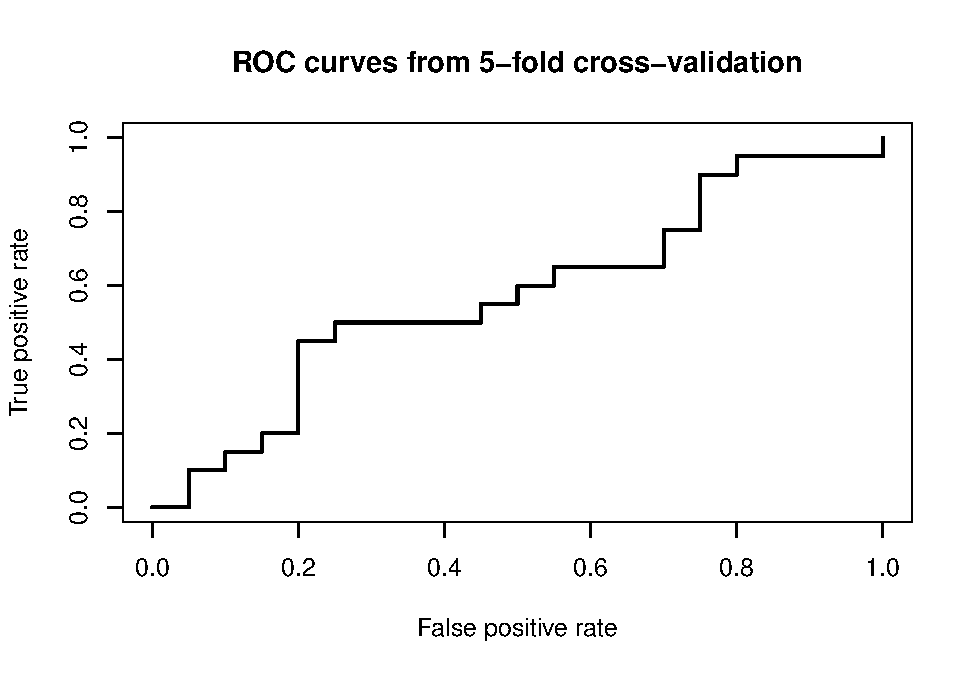
\includegraphics{final_GCM_files/figure-latex/unnamed-chunk-10-1.pdf}
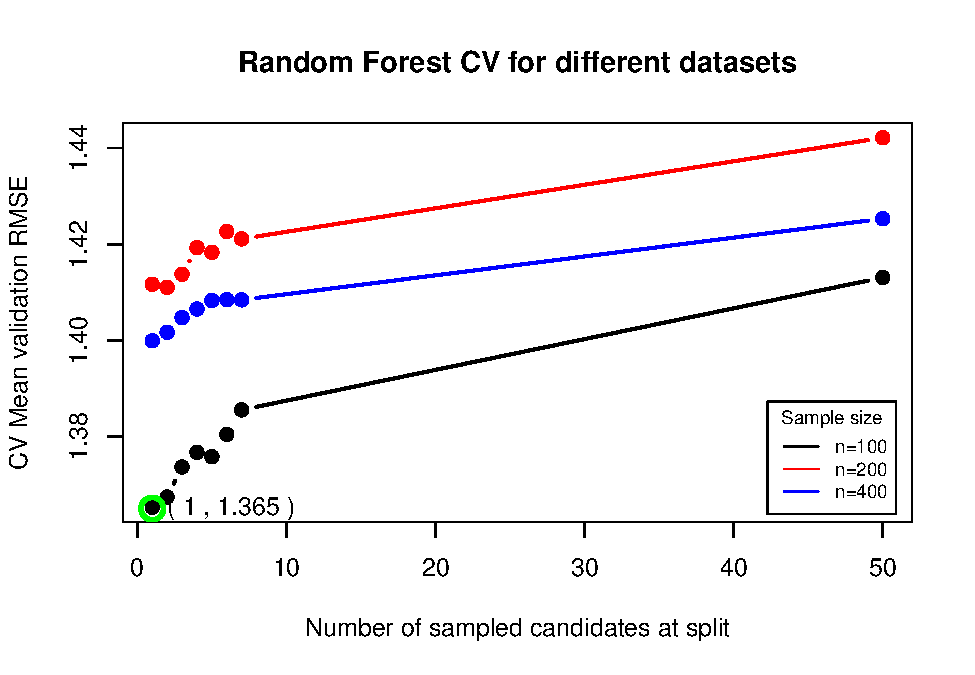
\includegraphics{final_GCM_files/figure-latex/unnamed-chunk-10-2.pdf}
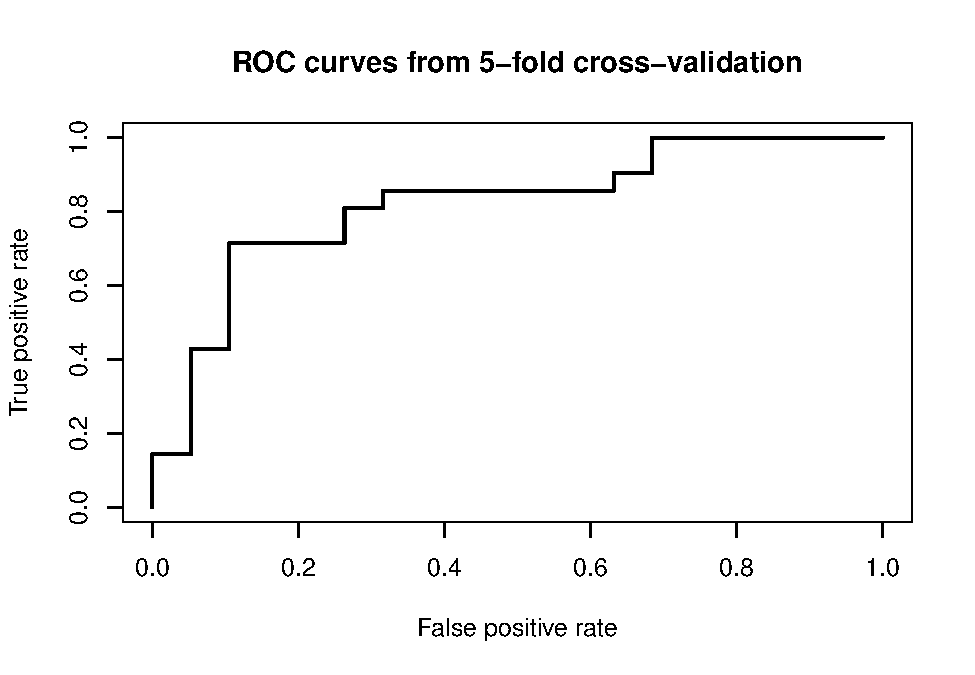
\includegraphics{final_GCM_files/figure-latex/unnamed-chunk-10-3.pdf}
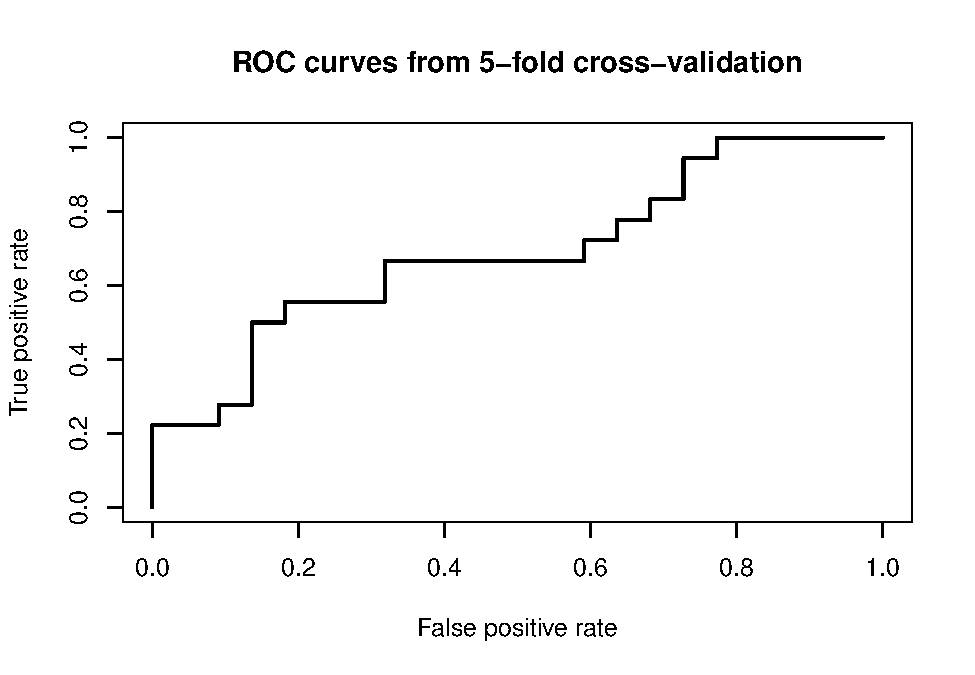
\includegraphics{final_GCM_files/figure-latex/unnamed-chunk-10-4.pdf}
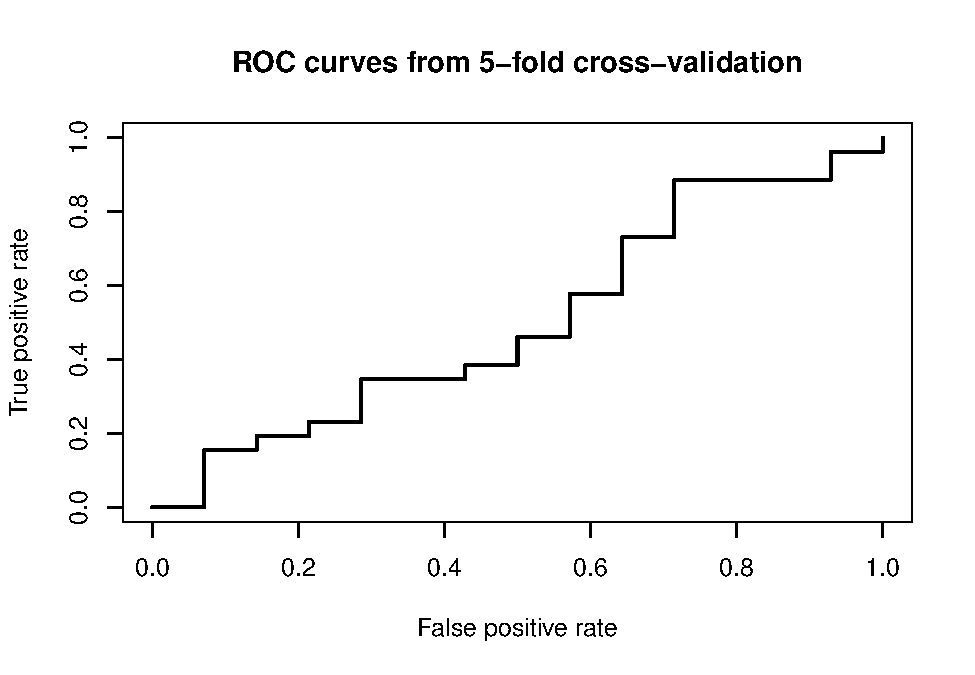
\includegraphics{final_GCM_files/figure-latex/unnamed-chunk-10-5.pdf}

\begin{Shaded}
\begin{Highlighting}[]
\CommentTok{\# this way seems to be the correct one}
\NormalTok{pred }\OtherTok{\textless{}{-}} \FunctionTok{prediction}\NormalTok{(Y\_pred, Y)}
\NormalTok{perf }\OtherTok{\textless{}{-}} \FunctionTok{performance}\NormalTok{(pred,}\StringTok{\textquotesingle{}tpr\textquotesingle{}}\NormalTok{,}\StringTok{\textquotesingle{}fpr\textquotesingle{}}\NormalTok{)}


\FunctionTok{plot}\NormalTok{(perf,}
     \AttributeTok{lwd=}\DecValTok{2}\NormalTok{,}
     \AttributeTok{main=}\StringTok{\textquotesingle{}ROC curves from 5{-}fold cross{-}validation\textquotesingle{}}\NormalTok{)}
\end{Highlighting}
\end{Shaded}

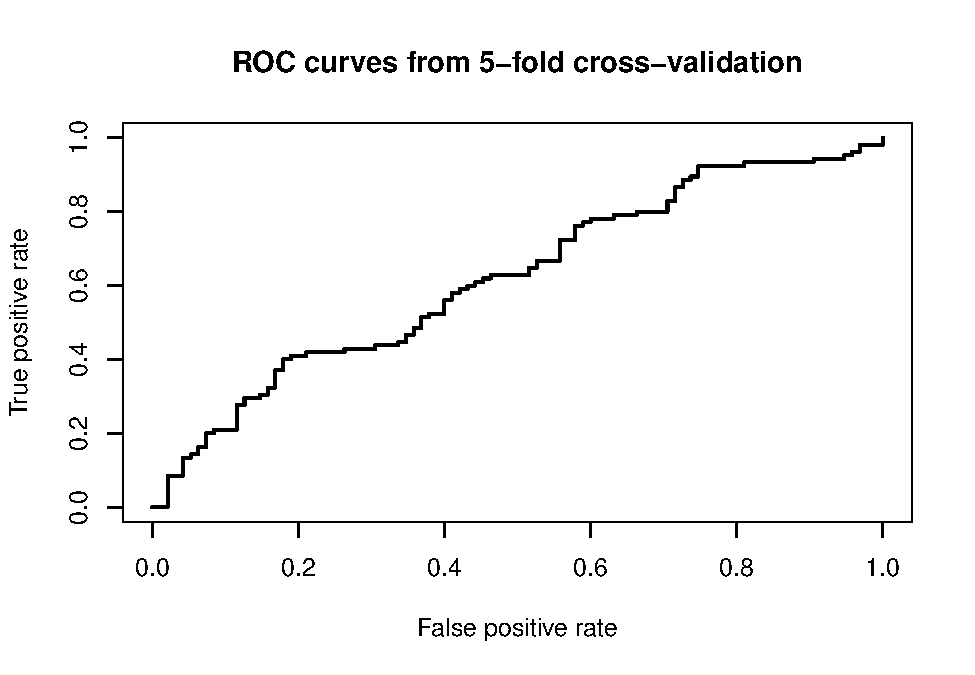
\includegraphics{final_GCM_files/figure-latex/unnamed-chunk-10-6.pdf}

\begin{Shaded}
\begin{Highlighting}[]
\CommentTok{\# print best threshold}
\CommentTok{\# show diagonal}

\StringTok{"For your best model, use 5{-}fold CV (same folds as in problem 4a) to construct the ROC curve plot. Your}
\StringTok{vector of predicted values for the ROC curve plot should be produced by training the best model on subset}
\StringTok{Ti and predicting on Vi. To get the entire vector of predicted values, put the 5 vectors of predicted values}
\StringTok{into a single vector; then compare vs truth (the whole vector Y ) proceeding as with the usual ROC curve}
\StringTok{plot construction (reuse the code examples from the ISLR book)."}
\end{Highlighting}
\end{Shaded}

\begin{verbatim}
## [1] "For your best model, use 5-fold CV (same folds as in problem 4a) to construct the ROC curve plot. Your\nvector of predicted values for the ROC curve plot should be produced by training the best model on subset\nTi and predicting on Vi. To get the entire vector of predicted values, put the 5 vectors of predicted values\ninto a single vector; then compare vs truth (the whole vector Y ) proceeding as with the usual ROC curve\nplot construction (reuse the code examples from the ISLR book)."
\end{verbatim}

\hypertarget{problem-5}{%
\section{Problem 5}\label{problem-5}}

\begin{Shaded}
\begin{Highlighting}[]
\NormalTok{p}\OtherTok{=}\DecValTok{50}
\NormalTok{n }\OtherTok{=} \FunctionTok{nrow}\NormalTok{(prob5.df)}
\NormalTok{test\_df }\OtherTok{=}\NormalTok{ prob5.df[}\DecValTok{401}\SpecialCharTok{:}\DecValTok{800}\NormalTok{,]}
\NormalTok{data\_set\_vec }\OtherTok{=} \FunctionTok{c}\NormalTok{(}\DecValTok{100}\NormalTok{, }\DecValTok{200}\NormalTok{, }\DecValTok{400}\NormalTok{)}
\NormalTok{k\_max }\OtherTok{=} \DecValTok{5}

\CommentTok{\# loop through sets of data}
\ControlFlowTok{for}\NormalTok{(set }\ControlFlowTok{in}\NormalTok{ data\_set\_vec)\{}
  \CommentTok{\# specify training data set}
\NormalTok{  train\_df }\OtherTok{=}\NormalTok{ prob5.df[}\DecValTok{1}\SpecialCharTok{:}\NormalTok{set,]}
  \CommentTok{\# perform 5{-}fold CV}
\NormalTok{  set\_n }\OtherTok{=} \FunctionTok{nrow}\NormalTok{(train\_df)}
\NormalTok{  inds.part }\OtherTok{=} \FunctionTok{myCVids}\NormalTok{(set\_n, }\DecValTok{5}\NormalTok{, }\AttributeTok{seed=}\DecValTok{0}\NormalTok{)}
\NormalTok{  lr\_rmse\_vec }\OtherTok{=} \FunctionTok{c}\NormalTok{()}
\NormalTok{  rf\_rmse\_vec }\OtherTok{=} \FunctionTok{c}\NormalTok{()}
\NormalTok{  gbm\_rmse\_vec }\OtherTok{=} \FunctionTok{c}\NormalTok{()}
  \ControlFlowTok{for}\NormalTok{(k }\ControlFlowTok{in} \FunctionTok{seq}\NormalTok{(}\DecValTok{1}\SpecialCharTok{:}\NormalTok{k\_max))\{}
\NormalTok{    isk }\OtherTok{=}\NormalTok{ (inds.part }\SpecialCharTok{==}\NormalTok{ k)}
\NormalTok{    valid.k }\OtherTok{=} \FunctionTok{which}\NormalTok{(isk)}
\NormalTok{    train.k }\OtherTok{=} \FunctionTok{which}\NormalTok{(}\SpecialCharTok{!}\NormalTok{isk)}
\NormalTok{    cv\_train\_df }\OtherTok{=}\NormalTok{ train\_df[train.k,]}
\NormalTok{    cv\_valid\_df }\OtherTok{=}\NormalTok{ train\_df[valid.k,]}
\NormalTok{    x\_cv\_train\_df }\OtherTok{=} \FunctionTok{model.matrix}\NormalTok{(Y}\SpecialCharTok{\textasciitilde{}}\NormalTok{., cv\_train\_df )[,}\SpecialCharTok{{-}}\DecValTok{1}\NormalTok{]}
\NormalTok{    y\_cv\_train\_df }\OtherTok{=}\NormalTok{ cv\_train\_df}\SpecialCharTok{$}\NormalTok{Y}
\NormalTok{    x\_cv\_valid\_df }\OtherTok{=} \FunctionTok{model.matrix}\NormalTok{(Y}\SpecialCharTok{\textasciitilde{}}\NormalTok{., cv\_valid\_df )[,}\SpecialCharTok{{-}}\DecValTok{1}\NormalTok{]}
\NormalTok{    y\_cv\_valid\_df }\OtherTok{=}\NormalTok{ cv\_valid\_df}\SpecialCharTok{$}\NormalTok{Y}
    
    \CommentTok{\# train LR}
    \FunctionTok{set.seed}\NormalTok{(}\DecValTok{0}\NormalTok{)}
\NormalTok{    lasso\_reg.fit }\OtherTok{=} \FunctionTok{glmnet}\NormalTok{(x\_cv\_train\_df,y\_cv\_train\_df, }\AttributeTok{alpha=}\DecValTok{1}\NormalTok{)}
    
    \CommentTok{\# train RF}
    \FunctionTok{set.seed}\NormalTok{(}\DecValTok{0}\NormalTok{)}
\NormalTok{    rf.fit }\OtherTok{=} \FunctionTok{randomForest}\NormalTok{(Y}\SpecialCharTok{\textasciitilde{}}\NormalTok{., }
                          \AttributeTok{data=}\NormalTok{cv\_train\_df, }
                          \AttributeTok{mtry=}\FunctionTok{c}\NormalTok{(}\DecValTok{1}\SpecialCharTok{:}\DecValTok{7}\NormalTok{,}\DecValTok{50}\NormalTok{),}
                          \AttributeTok{ntree=}\DecValTok{500}\NormalTok{,}
                          \AttributeTok{importance=}\ConstantTok{TRUE}\NormalTok{)}
    
    \CommentTok{\# train GBM}
    \FunctionTok{set.seed}\NormalTok{(}\DecValTok{0}\NormalTok{)}
\NormalTok{    gbm.fit }\OtherTok{=} \FunctionTok{gbm}\NormalTok{(Y}\SpecialCharTok{\textasciitilde{}}\NormalTok{., }
                  \AttributeTok{data=}\NormalTok{cv\_train\_df,}
                  \AttributeTok{distribution=}\StringTok{"gaussian"}\NormalTok{,}
                  \AttributeTok{n.trees=}\DecValTok{1000}\NormalTok{,}
                  \AttributeTok{shrinkage=}\FloatTok{0.01}\NormalTok{, }
                  \AttributeTok{interaction.depth=}\DecValTok{7}\NormalTok{) }\CommentTok{\# use 1:7 or test all or just one (7)}
    
    \CommentTok{\# eval LR}
\NormalTok{    lr\_pred }\OtherTok{=} \FunctionTok{predict}\NormalTok{(lasso\_reg.fit, x\_cv\_valid\_df)}
\NormalTok{    lr\_rmse }\OtherTok{=} \FunctionTok{sqrt}\NormalTok{(}\FunctionTok{mean}\NormalTok{((y\_cv\_valid\_df }\SpecialCharTok{{-}}\NormalTok{ lr\_pred)}\SpecialCharTok{\^{}}\DecValTok{2}\NormalTok{))}
\NormalTok{    lr\_rmse\_vec }\OtherTok{=} \FunctionTok{c}\NormalTok{(lr\_rmse\_vec, lr\_rmse)}
    
    \CommentTok{\# eval RF}
\NormalTok{    rf\_pred }\OtherTok{=} \FunctionTok{predict}\NormalTok{(rf.fit, cv\_valid\_df)}
\NormalTok{    rf\_rmse }\OtherTok{=} \FunctionTok{sqrt}\NormalTok{(}\FunctionTok{mean}\NormalTok{((y\_cv\_train\_df }\SpecialCharTok{{-}}\NormalTok{ rf\_pred)}\SpecialCharTok{\^{}}\DecValTok{2}\NormalTok{))}
\NormalTok{    rf\_rmse\_vec }\OtherTok{=} \FunctionTok{c}\NormalTok{(rf\_rmse\_vec, rf\_rmse)}
    
    \CommentTok{\# eval GBM}
\NormalTok{    gbm\_pred }\OtherTok{=} \FunctionTok{predict}\NormalTok{(gbm.fit, cv\_valid\_df)}
\NormalTok{    gbm\_rmse }\OtherTok{=} \FunctionTok{sqrt}\NormalTok{(}\FunctionTok{mean}\NormalTok{((y\_cv\_train\_df }\SpecialCharTok{{-}}\NormalTok{ gbm\_pred)}\SpecialCharTok{\^{}}\DecValTok{2}\NormalTok{))}
\NormalTok{    gbm\_rmse\_vec }\OtherTok{=} \FunctionTok{c}\NormalTok{(gbm\_rmse\_vec, gbm\_rmse)}
    
\NormalTok{  \}}
  \FunctionTok{print}\NormalTok{(set)}
  \FunctionTok{print}\NormalTok{(}\FunctionTok{mean}\NormalTok{(lr\_rmse\_vec))}
  \FunctionTok{print}\NormalTok{(}\FunctionTok{mean}\NormalTok{(rf\_rmse\_vec))}
  \FunctionTok{print}\NormalTok{(}\FunctionTok{mean}\NormalTok{(gbm\_rmse\_vec))}
  \FunctionTok{print}\NormalTok{(}\StringTok{"\_\_\_\_\_\_\_\_\_\_\_\_"}\NormalTok{)}
  
  
  
\NormalTok{\}}
\end{Highlighting}
\end{Shaded}

\begin{verbatim}
## [1] 100
## [1] 1.98515
## [1] 1.365293
## [1] 1.566195
## [1] "____________"
## [1] 200
## [1] 1.678889
## [1] 1.411676
## [1] 1.536651
## [1] "____________"
## [1] 400
## [1] 1.468838
## [1] 1.399912
## [1] 1.482933
## [1] "____________"
\end{verbatim}

\begin{Shaded}
\begin{Highlighting}[]
\CommentTok{\# find parameters that have to get tuned and tune for them. }
\CommentTok{\# plots should be tuning parameter and cv rmse}
\CommentTok{\# use cv as used to tune parameters in Q3}
\CommentTok{\# calcualte test and cv RMSE and print in table }

\CommentTok{\# Discuss what you expect: (i) as training sample size increases but the test  }
\CommentTok{\# sample is held fixed; (ii) training}
\CommentTok{\# set is held fixed but the test sample size increases.}


\StringTok{"For each method, report 3 CV RMSE curves (one curve for each n=100,200 and 400), overlaid on the}
\StringTok{same plot. Mark the optimal value of the CV RMSE and the corresponding value of the tuning parameter.}
\StringTok{Additionally, report the 3{-}by{-}6 matrix with rows corresponding to the three ML methods and columns}
\StringTok{corresponding to the CV RMSE and test RMSE for each value of n for model with parameters chosen by}
\StringTok{CV. (I.e., two RMSE values for n = 100, then the two RMSE values for n = 200, etc.) The CV RMSE}
\StringTok{will be computed from the training data only. The test RMSE should be computed by fitting the model}
\StringTok{on the entire training dataset with parameters determined by the CV; then this model is used to predict}
\StringTok{on the test set.}
\StringTok{Briefly discuss your findings; particularly, as n increases.}
\StringTok{For RF and GBM, report and discuss variable importance (for the best models).}
\StringTok{Discuss what you expect: (i) as training sample size increases but the test sample is held fixed; (ii) training}
\StringTok{set is held fixed but the test sample size increases."}
\end{Highlighting}
\end{Shaded}

\begin{verbatim}
## [1] "For each method, report 3 CV RMSE curves (one curve for each n=100,200 and 400), overlaid on the\nsame plot. Mark the optimal value of the CV RMSE and the corresponding value of the tuning parameter.\nAdditionally, report the 3-by-6 matrix with rows corresponding to the three ML methods and columns\ncorresponding to the CV RMSE and test RMSE for each value of n for model with parameters chosen by\nCV. (I.e., two RMSE values for n = 100, then the two RMSE values for n = 200, etc.) The CV RMSE\nwill be computed from the training data only. The test RMSE should be computed by fitting the model\non the entire training dataset with parameters determined by the CV; then this model is used to predict\non the test set.\nBriefly discuss your findings; particularly, as n increases.\nFor RF and GBM, report and discuss variable importance (for the best models).\nDiscuss what you expect: (i) as training sample size increases but the test sample is held fixed; (ii) training\nset is held fixed but the test sample size increases."
\end{verbatim}

\begin{Shaded}
\begin{Highlighting}[]
\CommentTok{\# generate additional 50 features}
\NormalTok{data\_df }\OtherTok{=} \FunctionTok{data.frame}\NormalTok{(prob5.df, }\FunctionTok{matrix}\NormalTok{( }\FunctionTok{rnorm}\NormalTok{(n}\SpecialCharTok{*}\DecValTok{50}\NormalTok{,}\AttributeTok{mean=}\DecValTok{0}\NormalTok{,}\AttributeTok{sd=}\DecValTok{1}\NormalTok{), n, }\DecValTok{50}\NormalTok{))}

\CommentTok{\# repeat 5 and see effect}

\CommentTok{\# What do you expect to happen to the predictive performance of }
\CommentTok{\# the methods?}
\end{Highlighting}
\end{Shaded}

\hypertarget{problem-6}{%
\section{Problem 6}\label{problem-6}}

\begin{Shaded}
\begin{Highlighting}[]
\CommentTok{\# define data}
\NormalTok{p }\OtherTok{=}\DecValTok{20}
\NormalTok{n }\OtherTok{=} \DecValTok{200}
\NormalTok{train\_df }\OtherTok{=}\NormalTok{ prob6.df[}\DecValTok{1}\SpecialCharTok{:}\DecValTok{200}\NormalTok{,]}
\NormalTok{test\_df }\OtherTok{=}\NormalTok{ prob6.df[}\DecValTok{201}\SpecialCharTok{:}\DecValTok{400}\NormalTok{,]}

\CommentTok{\# 5{-}fold validation}
\NormalTok{inds.part }\OtherTok{=} \FunctionTok{myCVids}\NormalTok{(n, }\DecValTok{5}\NormalTok{, }\AttributeTok{seed=}\DecValTok{0}\NormalTok{)}
\NormalTok{svm\_rmse\_vec }\OtherTok{=} \FunctionTok{c}\NormalTok{()}
\NormalTok{rf\_rmse\_vec }\OtherTok{=} \FunctionTok{c}\NormalTok{()}
\NormalTok{gbm\_rmse\_vec }\OtherTok{=} \FunctionTok{c}\NormalTok{()}
\ControlFlowTok{for}\NormalTok{(k }\ControlFlowTok{in} \FunctionTok{seq}\NormalTok{(}\DecValTok{1}\SpecialCharTok{:}\NormalTok{k\_max))\{}
\NormalTok{  isk }\OtherTok{=}\NormalTok{ (inds.part }\SpecialCharTok{==}\NormalTok{ k)}
\NormalTok{  valid.k }\OtherTok{=} \FunctionTok{which}\NormalTok{(isk)}
\NormalTok{  train.k }\OtherTok{=} \FunctionTok{which}\NormalTok{(}\SpecialCharTok{!}\NormalTok{isk)}
\NormalTok{  cv\_train\_df }\OtherTok{=}\NormalTok{ train\_df[train.k,]}
\NormalTok{  cv\_valid\_df }\OtherTok{=}\NormalTok{ train\_df[valid.k,]}
\NormalTok{  y\_cv\_valid\_df }\OtherTok{=}\NormalTok{ cv\_valid\_df}\SpecialCharTok{$}\NormalTok{Y}
  
  \CommentTok{\# train SVM}
  \FunctionTok{set.seed}\NormalTok{(}\DecValTok{0}\NormalTok{)}
\NormalTok{  svm.fit }\OtherTok{=} \FunctionTok{svm}\NormalTok{(Y}\SpecialCharTok{\textasciitilde{}}\NormalTok{., }
                \AttributeTok{data=}\NormalTok{cv\_train\_df, }
                \AttributeTok{kernel=}\StringTok{"radial"}\NormalTok{, }
                \AttributeTok{gamma=}\DecValTok{1}\NormalTok{,}
                \AttributeTok{cost=}\DecValTok{1}\NormalTok{,}
                \AttributeTok{type=}\StringTok{"C"}\NormalTok{)}
  
  \CommentTok{\# train RF}
  \FunctionTok{set.seed}\NormalTok{(}\DecValTok{0}\NormalTok{)}
\NormalTok{  rf.fit }\OtherTok{=} \FunctionTok{randomForest}\NormalTok{(}\FunctionTok{as.factor}\NormalTok{(Y)}\SpecialCharTok{\textasciitilde{}}\NormalTok{., }
                        \AttributeTok{data=}\NormalTok{cv\_train\_df, }
                        \AttributeTok{mtry=}\FunctionTok{c}\NormalTok{(}\DecValTok{1}\SpecialCharTok{:}\DecValTok{7}\NormalTok{,}\DecValTok{50}\NormalTok{),}
                        \AttributeTok{ntree=}\DecValTok{500}\NormalTok{,}
                        \AttributeTok{importance=}\ConstantTok{TRUE}\NormalTok{)}
  
  \CommentTok{\# train GBM}
  \FunctionTok{set.seed}\NormalTok{(}\DecValTok{0}\NormalTok{)}
\NormalTok{  gbm.fit }\OtherTok{=} \FunctionTok{gbm}\NormalTok{(Y}\SpecialCharTok{\textasciitilde{}}\NormalTok{., }
                \AttributeTok{data=}\NormalTok{cv\_train\_df,}
                \AttributeTok{distribution=}\StringTok{"bernoulli"}\NormalTok{,}
                \AttributeTok{n.trees=}\DecValTok{1000}\NormalTok{,}
                \AttributeTok{shrinkage=}\FloatTok{0.01}\NormalTok{, }
                \AttributeTok{interaction.depth=}\DecValTok{7}\NormalTok{) }\CommentTok{\# use 1:7 or test all or just one (7)}
  
  \CommentTok{\# eval SVM}
\NormalTok{  svm\_pred }\OtherTok{=} \FunctionTok{predict}\NormalTok{(svm.fit, cv\_valid\_df)}
  \CommentTok{\# svm\_rmse\_vec = c(svm\_rmse\_vec, svm\_rmse)}
  
  \CommentTok{\# eval RF}
\NormalTok{  rf\_pred }\OtherTok{=} \FunctionTok{predict}\NormalTok{(rf.fit, cv\_valid\_df)}
  \CommentTok{\# rf\_rmse\_vec = c(rf\_rmse\_vec, rf\_rmse)}
  
  \CommentTok{\# eval GBM}
\NormalTok{  gbm\_pred }\OtherTok{=} \FunctionTok{predict}\NormalTok{(gbm.fit, cv\_valid\_df)}
  \CommentTok{\# needs a threshold}
  \CommentTok{\# gbm\_rmse\_vec = c(gbm\_rmse\_vec, gbm\_rmse)}
  
\NormalTok{\}}
\end{Highlighting}
\end{Shaded}

\begin{verbatim}
## Using 1000 trees...
## 
## Using 1000 trees...
## 
## Using 1000 trees...
## 
## Using 1000 trees...
## 
## Using 1000 trees...
\end{verbatim}

\begin{Shaded}
\begin{Highlighting}[]
\CommentTok{\# print(mean(svm\_rmse\_vec))}
\CommentTok{\# print(mean(rf\_rmse\_vec))}
\CommentTok{\# print(mean(gbm\_rmse\_vec))}
\FunctionTok{print}\NormalTok{(}\StringTok{"\_\_\_\_\_\_\_\_\_\_\_\_"}\NormalTok{)}
\end{Highlighting}
\end{Shaded}

\begin{verbatim}
## [1] "____________"
\end{verbatim}

\begin{Shaded}
\begin{Highlighting}[]
\StringTok{"For each method, report CV misclassification error rate (MER) curves; this will be computed without using test data and used to select optimal tuning parameter values. }

\StringTok{Additionally, report the test MER for each classifier with the parameters chosen by CV (the entire training dataset to train the model with this set of tuning parameters, then predictions are made for the test data to determine MER).}

\StringTok{Lastly, overlay on the same plot ROCR curves for the three classifiers (with optimal tuning parameters). Here, the ROCR curves will be constructed using test data.}

\StringTok{Briefly discuss.}
\StringTok{"}
\end{Highlighting}
\end{Shaded}

\begin{verbatim}
## [1] "For each method, report CV misclassification error rate (MER) curves; this will be computed without using test data and used to select optimal tuning parameter values. \n\nAdditionally, report the test MER for each classifier with the parameters chosen by CV (the entire training dataset to train the model with this set of tuning parameters, then predictions are made for the test data to determine MER).\n\nLastly, overlay on the same plot ROCR curves for the three classifiers (with optimal tuning parameters). Here, the ROCR curves will be constructed using test data.\n\nBriefly discuss.\n"
\end{verbatim}

\end{document}
